% =====================================================================
%  Chapter 17: Exterior Derivatives: Gradient, Curl, and Divergence Revisited
% =====================================================================

\chapter{Exterior Derivatives: Gradient, Curl, and Divergence Revisited}
\label{ch:17}

Chapter \ref{ch:16} ended with a missing operation.  We can integrate \(0\)-forms,
\(1\)-forms, \(2\)-forms, and \(3\)-forms.  We can pull them back, wedge them, and
keep track of orientation.  But every boundary theorem we have seen involves one more
thing: a derivative.

For a function, the derivative is already familiar:
\[
    f \longmapsto df.
\]
Now the same symbol \(d\) will act on every kind of form:
\[
    0\text{-forms}\longrightarrow 1\text{-forms},
\]
\[
    1\text{-forms}\longrightarrow 2\text{-forms},
\]
\[
    2\text{-forms}\longrightarrow 3\text{-forms}.
\]

The operation is called the \emph{exterior derivative}.  Its job is to raise degree by
one.  In the old vector language, it appears as gradient, curl, and divergence.  In the
language of forms, those three operations are one operation seen at three different
degrees.

\section{The exterior derivative of a \texorpdfstring{\(0\)}{0}-form}
\label{sec:17.1}

A \(0\)-form is a function.  So the first case of the exterior derivative is the one we
already know:
\[
    f \longmapsto df.
\]
But now \(df\) is not just a symbol from single-variable calculus.  It is a \(1\)-form:
a rule that measures tangent vectors.

\subsection{From a function \texorpdfstring{\(f\)}{f} to its differential
\texorpdfstring{\(df\)}{df}}

Picture a metal plate on a laboratory table.  The point \((x,y)\) gives a location on the
plate, measured in centimeters.  The temperature is modeled by
\[
    T(x,y)=18+4x-y-\frac12x^2+\frac13xy.
\]
At the point
\[
    P=(2,3),
\]
the temperature is
\[
    T(2,3)=25.
\]

Now move a tiny amount
\[
    (\Delta x,\Delta y)=(h,k)
\]
from \(P\).  The new point is
\[
    (2+h,3+k).
\]
Substitute into \(T\):
\[
\begin{aligned}
T(2+h,3+k)
&=
18+4(2+h)-(3+k)-\frac12(2+h)^2
+\frac13(2+h)(3+k)\\
&=
25+3h-\frac13k+\frac13hk-\frac12h^2.
\end{aligned}
\]
So the temperature change is
\[
    T(2+h,3+k)-T(2,3)
    =
    3h-\frac13k+\frac13hk-\frac12h^2.
\]

The first-order part is
\[
    3h-\frac13k.
\]
The other terms,
\[
    \frac13hk-\frac12h^2,
\]
are smaller than the displacement when \((h,k)\) is very small.  So, near \(P\),
\[
    \Delta T\approx 3\,\Delta x-\frac13\,\Delta y.
\]

This linear measuring rule is the differential at \(P\):
\[
\boxed{
    dT_P=3\,dx-\frac13\,dy.
}
\]
It measures a tiny tangent vector
\[
    \mathbf v=(v_x,v_y)
\]
by
\[
    dT_P(\mathbf v)=3v_x-\frac13v_y.
\]

For example, suppose a small sensor is moving through \(P\) with velocity
\[
    \mathbf v=(2,-3)
\]
centimeters per second.  Then
\[
\begin{aligned}
    dT_P(\mathbf v)
    &=
    3(2)-\frac13(-3)\\
    &=
    7.
\end{aligned}
\]
So the sensor sees temperature increasing at
\[
    7^\circ\text{C per second}.
\]

\begin{figure}[h]
\centering
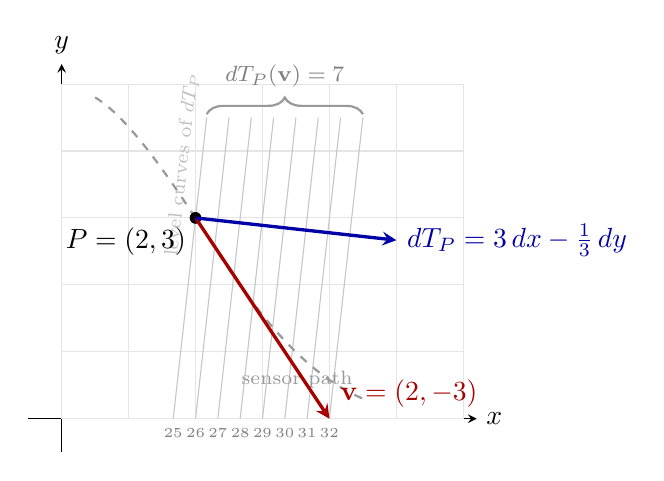
\begin{tikzpicture}[scale=0.85, >=stealth]
    \draw[->] (-0.5,0) -- (6.2,0) node[right] {\(x\)};
    \draw[->] (0,-0.5) -- (0,5.3) node[above] {\(y\)};

    \draw[gray!20, step=1] (0,0) grid (6,5);

    \coordinate (P) at (2,3);

    % 8 level curves representing T = 25 to T = 32
    % Based on the linear approximation: dT = 3dx - 1/3dy
    % Endpoints calculated at y=0 and y=4.5 to fit the grid perfectly
    \foreach \T in {25, 26, 27, 28, 29, 30, 31, 32} {
        \draw[gray!45] ({(3*\T - 60)/9}, 0) node[below, font=\tiny, text=gray] {\T} 
                    -- ({(3*\T - 55.5)/9}, 4.5);
    }
    
    \node[gray!50, font=\scriptsize, rotate=83.6] at (1.8, 3.8) {level curves of \(dT_P\)};

    % Curly brace indicating the total change of 7
    % (Requires \usetikzlibrary{decorations.pathreplacing} in preamble)
    \draw[decorate, decoration={brace, amplitude=6pt}, thick, gray!80]
        ({(3*25 - 55.5)/9}, 4.55) -- ({(3*32 - 55.5)/9}, 4.55)
        node[midway, above=6pt, text=gray, font=\footnotesize] {\(dT_P(\mathbf{v}) = 7\)};

    % Sensor path strictly tangent to v=(2,-3) at P
    \draw[dashed, thick, gray!80] (0.5, 4.8) 
        .. controls (1.0, 4.5) and (1.6, 3.6) .. (P) 
        .. controls (2.4, 2.4) and (3.3, 0.8) .. (4.5, 0.3) 
        node[above left, font=\scriptsize] {sensor path};

    \fill (P) circle[radius=2.5pt];
    \node[below left] at (P) {\(P=(2,3)\)};

    % Velocity vector v = (2,-3), drawn strictly to scale so it ends at (4,0)
    % This correctly lands exactly on the T=32 level curve
    \draw[->, very thick, red!65!black] (P) -- ++(2,-3)
        node[above right] {\(\mathbf{v}=(2,-3)\)};

    % The gradient vector representing dT_P = (3, -1/3)
    % Drawn geometrically accurately so it is strictly perpendicular to the level curves
    \draw[->, very thick, blue!65!black] (P) -- ++(3,-0.333)
        node[right] {\(dT_P=3\,dx-\frac{1}{3}\,dy\)};

\end{tikzpicture}
\caption{The differential \(dT_P\) is a \(1\)-form (a linear function), not a vector. Its true geometric representation is the family of parallel, evenly spaced level curves. The blue arrow is the gradient vector, acting as a visual proxy for the form; it points strictly perpendicular to the level curves in the direction of maximum increase. When the \(1\)-form evaluates a tangent vector \(\mathbf{v}\), it geometrically counts the number of level curves \(\mathbf{v}\) pierces. Here, the velocity vector \(\mathbf{v}\) crosses exactly \(7\) level increments, visualizing the algebraic result \(dT_P(\mathbf{v}) = 7\).}
\end{figure}

The calculation did two things at once.  It found the best linear approximation to the
change in temperature, and it produced a \(1\)-form.  That is exactly what \(d\) does to a
\(0\)-form.

\subsection{\texorpdfstring{\(df=f_x\,dx+f_y\,dy+f_z\,dz\)}{df = fx dx + fy dy + fz dz}}

In one variable, the differential is
\[
    df=f'(x)\,dx.
\]
That says a small change \(dx\) in the input produces the first-order output change
\[
    df\approx f'(x)\,dx.
\]

In two variables, there are two coordinate changes:
\[
    dx
    \qquad\text{and}\qquad
    dy.
\]
So a differentiable function
\[
    f(x,y)
\]
has differential
\[
\boxed{
    df=f_x\,dx+f_y\,dy.
}
\]

In three variables,
\[
\boxed{
    df=f_x\,dx+f_y\,dy+f_z\,dz.
}
\]

This is the first case of the exterior derivative.

\begin{definition}[Exterior derivative of a \(0\)-form]
Let \(f\) be a differentiable scalar function.

In the plane,
\[
\boxed{
    d f=f_x\,dx+f_y\,dy.
}
\]

In space,
\[
\boxed{
    d f=f_x\,dx+f_y\,dy+f_z\,dz.
}
\]

The form \(df\) is called the \emph{exterior derivative} of the \(0\)-form \(f\).
\end{definition}

When \(f\) has continuous first partial derivatives, this formula behaves smoothly from
point to point.  We will often say that \(f\) is \(C^1\).  That means:
\[
    f_x,\ f_y,\ f_z
    \quad\text{exist and are continuous}
\]
on the region under discussion.

The continuity condition is not just politeness.  Partial derivatives at a single point do
not automatically produce a true differential there.

\begin{example}[Why partial derivatives alone are not enough]
Define
\[
    f(x,y)=
    \begin{cases}
    \dfrac{xy}{\sqrt{x^2+y^2}}, & (x,y)\ne(0,0),\\[2mm]
    0, & (x,y)=(0,0).
    \end{cases}
\]
At the origin, the coordinate partial derivatives exist:
\[
    f_x(0,0)
    =
    \lim_{h\to0}\frac{f(h,0)-f(0,0)}{h}
    =
    0,
\]
and
\[
    f_y(0,0)
    =
    \lim_{k\to0}\frac{f(0,k)-f(0,0)}{k}
    =
    0.
\]
If those two numbers were enough, the differential at the origin would be
\[
    df_{(0,0)}=0.
\]

But along the diagonal path \((t,t)\),
\[
    f(t,t)=\frac{t^2}{\sqrt{2t^2}}=\frac{|t|}{\sqrt2}.
\]
The proposed linear approximation gives \(0\), and the error is
\[
    \frac{|t|}{\sqrt2}.
\]
Compare this to the size of the displacement:
\[
    \|(t,t)\|=\sqrt2\,|t|.
\]
The ratio is
\[
    \frac{|t|/\sqrt2}{\sqrt2\,|t|}=\frac12.
\]
It does not approach \(0\).

So \(f\) is not differentiable at the origin.  The partial derivatives exist there, but
there is no true differential \(df_{(0,0)}\).  A differential is a linear approximation to
all nearby directions at once, not only to the two coordinate directions.
\end{example}

This is the same warning from Chapter \ref{ch:7}, now in the language of forms.  The
form
\[
    f_x\,dx+f_y\,dy
\]
deserves to be called \(df\) at a point only when it really gives the first-order change of
\(f\) there.

\subsection{Relation to the gradient}

The differential \(df\) is a \(1\)-form.  The gradient \(\nabla f\) is a vector.

In Euclidean space, the dot product lets us translate between them.  If
\[
    f=f(x,y,z),
\]
then
\[
    df=f_x\,dx+f_y\,dy+f_z\,dz.
\]
On a tangent vector
\[
    \mathbf v=(v_x,v_y,v_z),
\]
this gives
\[
\begin{aligned}
    df_{\mathbf p}(\mathbf v)
    &=
    f_x(\mathbf p)v_x+f_y(\mathbf p)v_y+f_z(\mathbf p)v_z.
\end{aligned}
\]
The gradient vector is
\[
    \nabla f(\mathbf p)
    =
    \bigl(f_x(\mathbf p),f_y(\mathbf p),f_z(\mathbf p)\bigr).
\]
Therefore
\[
\boxed{
    df_{\mathbf p}(\mathbf v)
    =
    \nabla f(\mathbf p)\cdot \mathbf v.
}
\]

\begin{theorem}[The gradient represents \(df\) when a dot product is chosen]
Let \(f\) be differentiable at a point \(\mathbf p\in\mathbb R^3\), and use the usual
Euclidean dot product.  Then
\[
\boxed{
    df_{\mathbf p}(\mathbf v)=\nabla f(\mathbf p)\cdot\mathbf v
}
\]
for every tangent vector \(\mathbf v\).
\end{theorem}

\begin{proof}
Write
\[
    \mathbf v=(v_x,v_y,v_z).
\]
By the definition of \(df\),
\[
    df_{\mathbf p}(\mathbf v)
    =
    f_x(\mathbf p)v_x+f_y(\mathbf p)v_y+f_z(\mathbf p)v_z.
\]
By the definition of the dot product,
\[
    \nabla f(\mathbf p)\cdot\mathbf v
    =
    \bigl(f_x(\mathbf p),f_y(\mathbf p),f_z(\mathbf p)\bigr)
    \cdot
    (v_x,v_y,v_z),
\]
which is the same number.
\end{proof}

The theorem says the gradient and the differential contain the same coordinate
numbers in ordinary Euclidean space.  But they are different kinds of objects.

\[
\begin{array}{c|c|c}
\text{Object} & \text{Kind} & \text{What it does} \\ \hline
df & 1\text{-form} & \text{measures tangent vectors}\\[1mm]
\nabla f & \text{vector} & \text{points in the steepest direction}
\end{array}
\]

The dot product is the bridge between the two.  Without a dot product, the covector
\(df\) still makes sense.  The gradient vector needs that extra geometric structure.

\subsection{Directional derivatives from evaluating \texorpdfstring{\(df\)}{df}}

The differential answers the question:
\[
    \text{How fast does \(f\) change in this tangent direction?}
\]
If the direction is a unit vector \(\mathbf u\), then
\[
\boxed{
    D_{\mathbf u}f(\mathbf p)=df_{\mathbf p}(\mathbf u).
}
\]
Using the dot product, the same formula becomes
\[
\boxed{
    D_{\mathbf u}f(\mathbf p)=\nabla f(\mathbf p)\cdot\mathbf u.
}
\]

More generally, if \(\mathbf v\) is a velocity vector, not necessarily a unit vector, then
\[
    df_{\mathbf p}(\mathbf v)
\]
is the rate of change of \(f\) along motion with velocity \(\mathbf v\).

\begin{theorem}[Chain rule in differential-form language]
Let \(f\) be differentiable at \(\mathbf p\), and let
\[
    \mathbf r(t)
\]
be a differentiable curve with
\[
    \mathbf r(t_0)=\mathbf p.
\]
Then
\[
\boxed{
    \frac{d}{dt}f(\mathbf r(t))\bigg|_{t=t_0}
    =
    df_{\mathbf p}\bigl(\mathbf r'(t_0)\bigr).
}
\]
\end{theorem}

\begin{proof}
The curve supplies a tangent vector
\[
    \mathbf r'(t_0).
\]
The differential \(df_{\mathbf p}\) is the best linear measurement of how \(f\) changes
from \(\mathbf p\).  Applying that linear measurement to the curve's velocity gives the
first-order rate of change along the curve.  In coordinates, this is the chain rule:
\[
    \frac{d}{dt}f(x(t),y(t),z(t))
    =
    f_xx'(t)+f_yy'(t)+f_zz'(t).
\]
The right side is exactly
\[
    df_{\mathbf r(t)}(\mathbf r'(t)).
\]
\end{proof}

\begin{example}[A drone flying through a concentration field]
A drone flies through a room where the concentration of smoke is modeled by
\[
    C(x,y,z)=10+xz-y^2+\frac12x^2.
\]
The exterior derivative of \(C\) is
\[
    dC=(z+x)\,dx-2y\,dy+x\,dz.
\]
At the point
\[
    P=(1,2,3),
\]
this becomes
\[
    dC_P=4\,dx-4\,dy+dz.
\]

Suppose the drone passes through \(P\) with velocity
\[
    \mathbf v=(2,1,-3)
\]
meters per second.  Then the rate of change of the smoke concentration measured by
the drone is
\[
\begin{aligned}
    dC_P(\mathbf v)
    &=
    4(2)-4(1)+1(-3)\\
    &=
    1.
\end{aligned}
\]
So, at that instant, the concentration reading is increasing at
\[
    1
\]
concentration unit per second.

In gradient notation, this is the same computation:
\[
    \nabla C(P)=(4,-4,1),
\]
and
\[
    \nabla C(P)\cdot\mathbf v
    =
    (4,-4,1)\cdot(2,1,-3)=1.
\]
\end{example}

A \(0\)-form changes as we move along a curve, and \(df\) measures that change.  But a
\(1\)-form is already something we integrate along curves.  Its derivative should not
measure change along a single tangent vector.  It should measure what happens when we
walk around a tiny loop.  That is why the next form of \(d\) produces curl.

\section{The exterior derivative of a \texorpdfstring{\(1\)}{1}-form}
\label{sec:17.2}

Section \ref{sec:17.1} turned a function into a \(1\)-form:
\[
    f\longmapsto df.
\]
Now we ask what \(d\) does to a \(1\)-form.  The answer should be a \(2\)-form, because
the exterior derivative raises degree by one:
\[
    1\text{-form}\longrightarrow 2\text{-form}.
\]

Green's theorem already told us what to expect.  A \(1\)-form can be integrated around
a closed curve.  Its derivative should measure the circulation density inside the loop.

\subsection{Computing \texorpdfstring{\(d(P\,dx+Q\,dy)\)}{d(P dx + Q dy)} in the plane}

Recall the form from Chapter \ref{ch:14}:
\[
    \omega=(3-y)\,dx+2x\,dy.
\]
Around any small positively oriented rectangle, its circulation was
\[
    3\cdot\text{area}.
\]
So the derivative of \(\omega\) should be the \(2\)-form
\[
    3\,dx\wedge dy.
\]

The exterior derivative finds that number by differentiating the coefficient functions
and wedging with the coordinate forms.

The first term is
\[
    (3-y)\,dx.
\]
The coefficient has differential
\[
    d(3-y)=-dy.
\]
So
\[
    d\bigl((3-y)\,dx\bigr)
    =
    d(3-y)\wedge dx
    =
    (-dy)\wedge dx.
\]
Using
\[
    dy\wedge dx=-dx\wedge dy,
\]
we get
\[
    (-dy)\wedge dx=dx\wedge dy.
\]

The second term is
\[
    2x\,dy.
\]
The coefficient has differential
\[
    d(2x)=2\,dx.
\]
So
\[
    d(2x\,dy)
    =
    d(2x)\wedge dy
    =
    2\,dx\wedge dy.
\]

Add the two pieces:
\[
\begin{aligned}
    d\omega
    &=
    d\bigl((3-y)\,dx\bigr)+d(2x\,dy)\\
    &=
    dx\wedge dy+2\,dx\wedge dy\\
    &=
    3\,dx\wedge dy.
\end{aligned}
\]
This matches the rectangle calculation:
\[
    \oint_{\partial R}\omega
    =
    \iint_R 3\,dx\wedge dy.
\]

\begin{figure}[h]
\centering
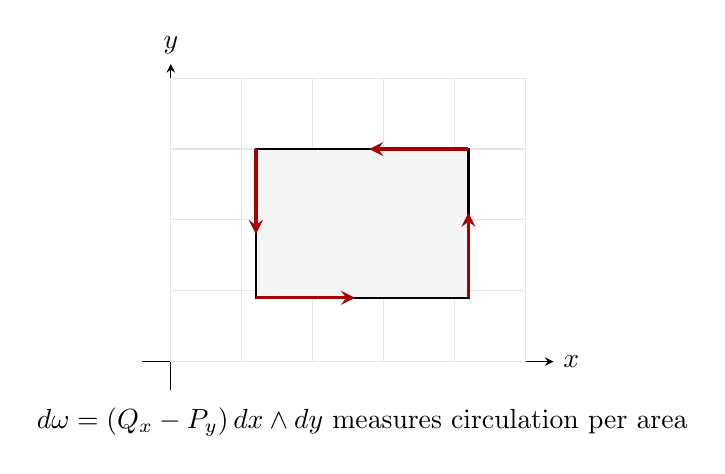
\begin{tikzpicture}[scale=0.9, >=stealth]
    \draw[->] (-0.4,0) -- (5.4,0) node[right] {\(x\)};
    \draw[->] (0,-0.4) -- (0,4.2) node[above] {\(y\)};

    \draw[gray!20, step=1] (0,0) grid (5,4);

    \draw[fill=gray!8, thick] (1.2,0.9) rectangle (4.2,3.0);

    \draw[->, very thick, red!65!black] (1.2,0.9) -- (2.6,0.9);
    \draw[->, very thick, red!65!black] (4.2,0.9) -- (4.2,2.1);
    \draw[->, very thick, red!65!black] (4.2,3.0) -- (2.8,3.0);
    \draw[->, very thick, red!65!black] (1.2,3.0) -- (1.2,1.8);

    \node at (2.7,-0.85)
        {\(\displaystyle d\omega=(Q_x-P_y)\,dx\wedge dy\) measures circulation per area};
\end{tikzpicture}
\caption{The exterior derivative of a plane \(1\)-form measures circulation density.}
\end{figure}

The same computation works for every plane \(1\)-form
\[
    \omega=P\,dx+Q\,dy.
\]

Since
\[
    dP=P_x\,dx+P_y\,dy
\]
and
\[
    dQ=Q_x\,dx+Q_y\,dy,
\]
we get
\[
\begin{aligned}
    d\omega
    &=
    dP\wedge dx+dQ\wedge dy\\
    &=
    (P_x\,dx+P_y\,dy)\wedge dx
    +
    (Q_x\,dx+Q_y\,dy)\wedge dy.
\end{aligned}
\]
Now use
\[
    dx\wedge dx=0,
    \qquad
    dy\wedge dy=0,
\]
and
\[
    dy\wedge dx=-dx\wedge dy.
\]
Then
\[
\begin{aligned}
    d\omega
    &=
    P_y\,dy\wedge dx+Q_x\,dx\wedge dy\\
    &=
    -P_y\,dx\wedge dy+Q_x\,dx\wedge dy\\
    &=
    (Q_x-P_y)\,dx\wedge dy.
\end{aligned}
\]

\begin{definition}[Exterior derivative of a plane \(1\)-form]
Let
\[
    \omega=P(x,y)\,dx+Q(x,y)\,dy
\]
be a \(1\)-form with \(C^1\) coefficient functions.  Its exterior derivative is the
\(2\)-form
\[
\boxed{
    d\omega=(Q_x-P_y)\,dx\wedge dy.
}
\]
\end{definition}

The coefficient
\[
    Q_x-P_y
\]
is the scalar curl from Chapter \ref{ch:14}.  So in the plane,
\[
\boxed{
    d(P\,dx+Q\,dy)
    =
    \operatorname{curl}_{\mathrm{plane}}(P,Q)\,dx\wedge dy.
}
\]

\begin{example}[A zero exterior derivative]
Let
\[
    \omega=(2x+y)\,dx+(x-3y)\,dy.
\]
Here
\[
    P=2x+y,
    \qquad
    Q=x-3y.
\]
Then
\[
    P_y=1,
    \qquad
    Q_x=1.
\]
Therefore
\[
    d\omega=(1-1)\,dx\wedge dy=0.
\]

This does not mean \(\omega\) itself is zero.  For example, at \((1,0)\),
\[
    \omega=2\,dx+dy.
\]
It means the local circulation density is zero.  Around very small loops, the leading
circulation cancels.
\end{example}

\subsection{Computing \texorpdfstring{\(d(P\,dx+Q\,dy+R\,dz)\)}%
{d(P dx + Q dy + R dz)} in space}

In space, a \(1\)-form has the shape
\[
    \omega=P\,dx+Q\,dy+R\,dz.
\]
Its exterior derivative should be a \(2\)-form.  Since \(2\)-forms in space have three
basic pieces,
\[
    dy\wedge dz,\qquad dz\wedge dx,\qquad dx\wedge dy,
\]
we should expect three coefficients.

Work through one example first.

Let
\[
    \omega=z^2\,dx+xz\,dy+y^2\,dz.
\]
Then
\[
    P=z^2,
    \qquad
    Q=xz,
    \qquad
    R=y^2.
\]
Differentiate the coefficients:
\[
    dP=2z\,dz,
\]
\[
    dQ=z\,dx+x\,dz,
\]
and
\[
    dR=2y\,dy.
\]
Now wedge each differential with its coordinate form:
\[
\begin{aligned}
    d\omega
    &=
    dP\wedge dx+dQ\wedge dy+dR\wedge dz\\
    &=
    (2z\,dz)\wedge dx
    +
    (z\,dx+x\,dz)\wedge dy
    +
    (2y\,dy)\wedge dz.
\end{aligned}
\]
Rewrite in the standard order
\[
    dy\wedge dz,\qquad dz\wedge dx,\qquad dx\wedge dy.
\]
We get
\[
\begin{aligned}
    d\omega
    &=
    2z\,dz\wedge dx
    +
    z\,dx\wedge dy
    +
    x\,dz\wedge dy
    +
    2y\,dy\wedge dz\\
    &=
    (2y-x)\,dy\wedge dz
    +
    2z\,dz\wedge dx
    +
    z\,dx\wedge dy.
\end{aligned}
\]
So
\[
\boxed{
    d\omega
    =
    (2y-x)\,dy\wedge dz
    +
    2z\,dz\wedge dx
    +
    z\,dx\wedge dy.
}
\]

The same pattern gives the general formula.

Let
\[
    \omega=P\,dx+Q\,dy+R\,dz.
\]
Then
\[
    d\omega=dP\wedge dx+dQ\wedge dy+dR\wedge dz.
\]
Use
\[
    dP=P_x\,dx+P_y\,dy+P_z\,dz,
\]
\[
    dQ=Q_x\,dx+Q_y\,dy+Q_z\,dz,
\]
and
\[
    dR=R_x\,dx+R_y\,dy+R_z\,dz.
\]
After deleting repeated wedges and reordering signs, we get
\[
\boxed{
    d\omega
    =
    (R_y-Q_z)\,dy\wedge dz
    +
    (P_z-R_x)\,dz\wedge dx
    +
    (Q_x-P_y)\,dx\wedge dy.
}
\]

\begin{definition}[Exterior derivative of a space \(1\)-form]
Let
\[
    \omega=P\,dx+Q\,dy+R\,dz
\]
be a \(1\)-form in space with \(C^1\) coefficient functions.  Its exterior derivative is
\[
\boxed{
    d\omega
    =
    (R_y-Q_z)\,dy\wedge dz
    +
    (P_z-R_x)\,dz\wedge dx
    +
    (Q_x-P_y)\,dx\wedge dy.
}
\]
\end{definition}

The coordinate forms themselves have zero exterior derivative:
\[
    d(dx)=d(dy)=d(dz)=0.
\]
The variation comes from the coefficient functions \(P,Q,R\), not from the constant
coordinate measuring rules.

\subsection{Curl hidden inside \texorpdfstring{\(d\omega\)}{d omega}}

The formula for \(d\omega\) looks familiar if we compare it with curl.

For a vector field
\[
    \mathbf F=(P,Q,R),
\]
the classical curl is
\[
\boxed{
    \nabla\times\mathbf F
    =
    (R_y-Q_z,\ P_z-R_x,\ Q_x-P_y).
}
\]
The exterior derivative of the work form
\[
    \omega=P\,dx+Q\,dy+R\,dz
\]
is
\[
\boxed{
    d\omega
    =
    (R_y-Q_z)\,dy\wedge dz
    +
    (P_z-R_x)\,dz\wedge dx
    +
    (Q_x-P_y)\,dx\wedge dy.
}
\]

So \(d\omega\) is the flux \(2\)-form associated with the curl vector field:
\[
\boxed{
    d\omega=\Phi_{\nabla\times\mathbf F}.
}
\]
Here
\[
    \Phi_{\mathbf G}
    =
    G_1\,dy\wedge dz+G_2\,dz\wedge dx+G_3\,dx\wedge dy
\]
is the flux form of a vector field \(\mathbf G=(G_1,G_2,G_3)\).

\begin{theorem}[Exterior derivative of a work form is curl as a flux form]
Let
\[
    \mathbf F=(P,Q,R)
\]
be a \(C^1\) vector field in space, and let
\[
    \omega_{\mathbf F}=P\,dx+Q\,dy+R\,dz
\]
be its work \(1\)-form.  Then
\[
\boxed{
    d\omega_{\mathbf F}=\Phi_{\nabla\times\mathbf F}.
}
\]
\end{theorem}

\begin{proof}
The flux form of
\[
    \nabla\times\mathbf F
    =
    (R_y-Q_z,\ P_z-R_x,\ Q_x-P_y)
\]
is
\[
    (R_y-Q_z)\,dy\wedge dz
    +
    (P_z-R_x)\,dz\wedge dx
    +
    (Q_x-P_y)\,dx\wedge dy.
\]
This is exactly the formula for
\[
    d(P\,dx+Q\,dy+R\,dz).
\]
\end{proof}

This theorem explains the word \emph{curl} in a clean way.  The curl is not a separate
mystery operation.  It is the exterior derivative of a \(1\)-form, read through the
three-dimensional flux-form dictionary.

\begin{example}[A rotating air flow in space]
Let
\[
    \mathbf F=(-y,\ x,\ z).
\]
Its work form is
\[
    \omega=-y\,dx+x\,dy+z\,dz.
\]
Compute \(d\omega\):
\[
    P=-y,\qquad Q=x,\qquad R=z.
\]
Then
\[
    R_y-Q_z=0-0=0,
\]
\[
    P_z-R_x=0-0=0,
\]
and
\[
    Q_x-P_y=1-(-1)=2.
\]
Therefore
\[
\boxed{
    d\omega=2\,dx\wedge dy.
}
\]
The curl vector is
\[
    \nabla\times\mathbf F=(0,0,2).
\]
The field rotates around the \(z\)-axis, and the exterior derivative records that
rotation as a \(2\)-form measuring \(xy\)-oriented surface pieces.
\end{example}

\subsection{Green's and Stokes' theorem previewed again}

In the plane, the formula
\[
    d(P\,dx+Q\,dy)=(Q_x-P_y)\,dx\wedge dy
\]
turns Green's theorem into the short statement
\[
\boxed{
    \int_{\partial R}\omega=\int_R d\omega.
}
\]
The left side is circulation around the boundary.  The right side is circulation density
added over the inside.

For example, with
\[
    \omega=(3-y)\,dx+2x\,dy,
\]
we found
\[
    d\omega=3\,dx\wedge dy.
\]
So Green's theorem says
\[
\boxed{
    \int_{\partial R}\omega
    =
    \int_R 3\,dx\wedge dy
    =
    3\,\operatorname{Area}(R)
}
\]
for every positively oriented plane region \(R\) to which the theorem applies.

In space, the same statement becomes Stokes' theorem:
\[
\boxed{
    \int_{\partial S}\omega=\int_S d\omega.
}
\]
Now \(S\) is an oriented surface, and \(\partial S\) is its oriented boundary curve.
The exterior derivative \(d\omega\) is the curl \(2\)-form.

\begin{example}[The same boundary with a curved surface]
Let
\[
    \omega=-y\,dx+x\,dy+z\,dz,
\]
so
\[
    d\omega=2\,dx\wedge dy.
\]
Let \(S\) be the upper hemisphere
\[
    x^2+y^2+z^2=1,\qquad z\ge0,
\]
oriented upward.  Its boundary is the unit circle in the \(xy\)-plane, oriented
counterclockwise as seen from above.

Stokes' theorem predicts
\[
    \int_{\partial S}\omega=\int_S 2\,dx\wedge dy.
\]
The form \(dx\wedge dy\) measures the signed \(xy\)-shadow of the surface.  The
upward-oriented upper hemisphere casts the unit disk as its positive shadow.  Therefore
\[
    \int_S 2\,dx\wedge dy=2\pi.
\]

Check the boundary integral directly.  Parametrize the boundary by
\[
    \mathbf r(t)=(\cos t,\sin t,0),
    \qquad
    0\le t\le2\pi.
\]
Then
\[
    dx=-\sin t\,dt,
    \qquad
    dy=\cos t\,dt,
    \qquad
    dz=0.
\]
So
\[
\begin{aligned}
    \mathbf r^*\omega
    &=
    -\sin t(-\sin t\,dt)+\cos t(\cos t\,dt)+0\\
    &=
    dt.
\end{aligned}
\]
Hence
\[
\boxed{
    \int_{\partial S}\omega=\int_0^{2\pi}dt=2\pi.
}
\]
The curved surface and the flat disk have the same boundary, and the same \(d\omega\)
accounts for the boundary circulation.
\end{example}

The hypotheses behind Green's and Stokes' theorem matter.  The form must be defined
and smooth on a region containing the surface or plane region we integrate over.  A
missing point can break the conclusion.

\begin{example}[A hidden singularity breaks the theorem]
Consider the \(1\)-form
\[
    \omega_0
    =
    \frac{-y}{x^2+y^2}\,dx
    +
    \frac{x}{x^2+y^2}\,dy.
\]
It is defined on
\[
    \mathbb R^2\setminus\{(0,0)\},
\]
not at the origin.

Away from the origin,
\[
    P=\frac{-y}{x^2+y^2},
    \qquad
    Q=\frac{x}{x^2+y^2}.
\]
A direct calculation gives
\[
    Q_x-P_y=0,
\]
so
\[
    d\omega_0=0
\]
wherever the form is defined.

Now integrate around the unit circle
\[
    C:\quad \mathbf r(t)=(\cos t,\sin t),
    \qquad 0\le t\le2\pi.
\]
On this circle,
\[
    x^2+y^2=1,
\]
so
\[
    \omega_0=-y\,dx+x\,dy.
\]
As before,
\[
    \mathbf r^*\omega_0=dt.
\]
Therefore
\[
\boxed{
    \int_C\omega_0=2\pi.
}
\]

If we pretended Green's theorem applied to the whole disk, we would get
\[
    \int_C\omega_0
    =
    \int_{\text{disk}}d\omega_0
    =
    0,
\]
which is false.  The problem is the missing origin.  The form is not defined on the
disk bounded by \(C\).

So the condition ``defined and smooth on the whole region'' is not a technical detail.
It prevents a singularity from hiding inside the boundary.
\end{example}

The exterior derivative has now turned functions into \(1\)-forms and \(1\)-forms into
\(2\)-forms:
\[
    f\longmapsto df,
    \qquad
    \omega\longmapsto d\omega.
\]
The next step is forced by the divergence theorem.  A flux \(2\)-form measures flow
through a surface.  Its derivative should measure source density inside a volume.  That
will be a \(3\)-form, and the old vector name for its coefficient is divergence.
\section{The exterior derivative of a \texorpdfstring{\(2\)}{2}-form}
\label{sec:17.3}

Section \ref{sec:17.2} turned a work \(1\)-form into a flux \(2\)-form:
\[
    \omega_{\mathbf F}
    \quad\longmapsto\quad
    d\omega_{\mathbf F}
    =
    \Phi_{\nabla\times\mathbf F}.
\]
A \(2\)-form is integrated over a surface.  So its derivative should be integrated over
a solid.  That means the next exterior derivative should measure source strength
inside volume.

\subsection{Computing
\texorpdfstring{\(d(P\,dy\wedge dz+Q\,dz\wedge dx+R\,dx\wedge dy)\)}%
{d(P dy dz + Q dz dx + R dx dy)}}

Picture air flowing through a sealed box.  The flux through the boundary tells us
whether more air is leaving than entering.  If more leaves than enters, something
inside acts like a source.  If more enters than leaves, something inside acts like a sink.

The flux \(2\)-form of a vector field
\[
    \mathbf F=(P,Q,R)
\]
is
\[
    \Phi_{\mathbf F}
    =
    P\,dy\wedge dz
    +
    Q\,dz\wedge dx
    +
    R\,dx\wedge dy.
\]
The three pieces measure flux through the three coordinate shadows:

\[
\begin{array}{c|c|c}
\text{Piece} & \text{Surface direction} & \text{Field component measured}\\ \hline
dy\wedge dz & yz\text{-oriented area} & x\text{-component }P\\[1mm]
dz\wedge dx & zx\text{-oriented area} & y\text{-component }Q\\[1mm]
dx\wedge dy & xy\text{-oriented area} & z\text{-component }R
\end{array}
\]

Start with the simple expanding field
\[
    \mathbf F(x,y,z)=(x,2y,3z).
\]
Its flux form is
\[
    \Phi=x\,dy\wedge dz+2y\,dz\wedge dx+3z\,dx\wedge dy.
\]
Chapter \ref{ch:15} computed the outward flux of this field through a rectangular box
and found
\[
    \text{outward flux}=6\cdot\text{volume}.
\]
So its exterior derivative should be
\[
    6\,dx\wedge dy\wedge dz.
\]

Now compute with \(d\).

For the first term,
\[
\begin{aligned}
d\bigl(x\,dy\wedge dz\bigr)
&=
dx\wedge dy\wedge dz.
\end{aligned}
\]
For the second term,
\[
\begin{aligned}
d\bigl(2y\,dz\wedge dx\bigr)
&=
2\,dy\wedge dz\wedge dx.
\end{aligned}
\]
The order
\[
    dy\wedge dz\wedge dx
\]
is a cyclic shift of
\[
    dx\wedge dy\wedge dz,
\]
so it has the same sign:
\[
    dy\wedge dz\wedge dx=dx\wedge dy\wedge dz.
\]
Thus
\[
    d\bigl(2y\,dz\wedge dx\bigr)
    =
    2\,dx\wedge dy\wedge dz.
\]

For the third term,
\[
\begin{aligned}
d\bigl(3z\,dx\wedge dy\bigr)
&=
3\,dz\wedge dx\wedge dy\\
&=
3\,dx\wedge dy\wedge dz.
\end{aligned}
\]
Again the order is cyclic, so the sign is positive.

Add the three pieces:
\[
\begin{aligned}
d\Phi
&=
dx\wedge dy\wedge dz
+
2\,dx\wedge dy\wedge dz
+
3\,dx\wedge dy\wedge dz\\
&=
6\,dx\wedge dy\wedge dz.
\end{aligned}
\]
So
\[
\boxed{
    d\Phi=6\,dx\wedge dy\wedge dz.
}
\]
The coefficient \(6\) is the source density.  Every small volume box has net outward
flux approximately
\[
    6\,\Delta V.
\]

\begin{figure}[h]
\centering
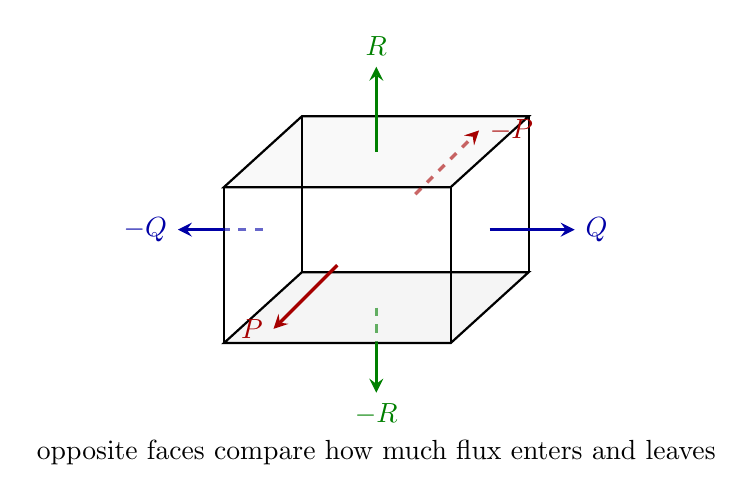
\begin{tikzpicture}[scale=0.9, >=stealth]
    \coordinate (O) at (0,0);
    \coordinate (A) at (3.2,0);
    \coordinate (B) at (4.3,1.0);
    \coordinate (C) at (1.1,1.0);
    \coordinate (D) at (0,2.2);
    \coordinate (E) at (3.2,2.2);
    \coordinate (F) at (4.3,3.2);
    \coordinate (G) at (1.1,3.2);

    \draw[fill=gray!8, thick] (O)--(A)--(B)--(C)--cycle;
    \draw[fill=gray!5, thick] (D)--(E)--(F)--(G)--cycle;
    \draw[thick] (O)--(D);
    \draw[thick] (A)--(E);
    \draw[thick] (B)--(F);
    \draw[thick] (C)--(G);

    % X-axis fluxes (P and -P) - Front and Back faces
    % Back face (hidden): -P points into the page (+x direction)
    \draw[->, very thick, red!65!black, dashed, draw opacity=0.6] (2.7,2.1) -- (3.6,3.0)
        node[right, text opacity=1] {\(-P\)};
    % Front face (visible): P points out of the page (-x direction)
    \draw[->, very thick, red!65!black] (1.6,1.1) -- (0.7,0.2)
        node[left] {\(P\)};

    % Y-axis fluxes (Q and -Q) - Right and Left faces
    % Left face (hidden): -Q points left (-y direction)
    \draw[very thick, blue!65!black, dashed, draw opacity=0.6] (0.55,1.6) -- (0,1.6);
    \draw[->, very thick, blue!65!black] (0,1.6) -- (-0.65,1.6)
        node[left] {\(-Q\)};
    % Right face (visible): Q points right (+y direction)
    \draw[->, very thick, blue!65!black] (3.75,1.6) -- (4.95,1.6)
        node[right] {\(Q\)};

    % Z-axis fluxes (R and -R) - Top and Bottom faces
    % Bottom face (hidden): -R points down (-z direction)
    \draw[very thick, green!50!black, dashed, draw opacity=0.6] (2.15,0.5) -- (2.15,0);
    \draw[->, very thick, green!50!black] (2.15,0) -- (2.15,-0.7)
        node[below] {\(-R\)};
    % Top face (visible): R points up (+z direction)
    \draw[->, very thick, green!50!black] (2.15,2.7) -- (2.15,3.9)
        node[above] {\(R\)};

    \node at (2.15,-1.55)
        {opposite faces compare how much flux enters and leaves};
\end{tikzpicture}
\caption{The exterior derivative of a flux \(2\)-form measures net outward flux per
unit volume.}
\end{figure}

The same calculation works for every flux \(2\)-form in space.

Let
\[
    \Phi=P\,dy\wedge dz+Q\,dz\wedge dx+R\,dx\wedge dy.
\]
Then
\[
    d\Phi
    =
    dP\wedge dy\wedge dz
    +
    dQ\wedge dz\wedge dx
    +
    dR\wedge dx\wedge dy.
\]
Use
\[
    dP=P_x\,dx+P_y\,dy+P_z\,dz.
\]
Only the \(P_x\,dx\) term survives, because
\[
    dy\wedge dy=0,
    \qquad
    dz\wedge dz=0.
\]
So
\[
    dP\wedge dy\wedge dz
    =
    P_x\,dx\wedge dy\wedge dz.
\]

Similarly,
\[
    dQ=Q_x\,dx+Q_y\,dy+Q_z\,dz.
\]
Only the \(Q_y\,dy\) term survives:
\[
\begin{aligned}
    dQ\wedge dz\wedge dx
    &=
    Q_y\,dy\wedge dz\wedge dx\\
    &=
    Q_y\,dx\wedge dy\wedge dz.
\end{aligned}
\]

Finally,
\[
    dR=R_x\,dx+R_y\,dy+R_z\,dz.
\]
Only the \(R_z\,dz\) term survives:
\[
\begin{aligned}
    dR\wedge dx\wedge dy
    &=
    R_z\,dz\wedge dx\wedge dy\\
    &=
    R_z\,dx\wedge dy\wedge dz.
\end{aligned}
\]

Therefore
\[
\boxed{
    d\Phi
    =
    (P_x+Q_y+R_z)\,dx\wedge dy\wedge dz.
}
\]

\begin{definition}[Exterior derivative of a space \(2\)-form]
Let
\[
    \Phi=P\,dy\wedge dz+Q\,dz\wedge dx+R\,dx\wedge dy
\]
be a \(2\)-form in space with \(C^1\) coefficient functions.  Its exterior derivative is
the \(3\)-form
\[
\boxed{
    d\Phi
    =
    (P_x+Q_y+R_z)\,dx\wedge dy\wedge dz.
}
\]
\end{definition}

The notation is compact, but the meaning is physical:

\[
\boxed{
    d(\text{flux form})=\text{source density volume form}.
}
\]

\subsection{Divergence hidden inside \texorpdfstring{\(d\Phi\)}{d Phi}}

For a vector field
\[
    \mathbf F=(P,Q,R),
\]
the classical divergence is
\[
\boxed{
    \nabla\cdot\mathbf F=P_x+Q_y+R_z.
}
\]
The flux form of \(\mathbf F\) is
\[
    \Phi_{\mathbf F}
    =
    P\,dy\wedge dz
    +
    Q\,dz\wedge dx
    +
    R\,dx\wedge dy.
\]
Taking its exterior derivative gives
\[
\boxed{
    d\Phi_{\mathbf F}
    =
    (\nabla\cdot\mathbf F)\,dx\wedge dy\wedge dz.
}
\]

\begin{theorem}[Exterior derivative of a flux form is divergence as a volume form]
Let
\[
    \mathbf F=(P,Q,R)
\]
be a \(C^1\) vector field in space, and let
\[
    \Phi_{\mathbf F}
    =
    P\,dy\wedge dz
    +
    Q\,dz\wedge dx
    +
    R\,dx\wedge dy
\]
be its flux \(2\)-form.  Then
\[
\boxed{
    d\Phi_{\mathbf F}
    =
    (\nabla\cdot\mathbf F)\,dx\wedge dy\wedge dz.
}
\]
\end{theorem}

\begin{proof}
The coefficient of \(d\Phi_{\mathbf F}\) is
\[
    P_x+Q_y+R_z,
\]
which is exactly
\[
    \nabla\cdot\mathbf F.
\]
\end{proof}

The theorem completes the promised dictionary:

\[
\begin{array}{c|c|c}
\text{Form} & \text{Exterior derivative} & \text{Classical name}\\ \hline
f & df & \text{gradient information}\\[1mm]
P\,dx+Q\,dy+R\,dz & d\omega & \text{curl flux form}\\[1mm]
P\,dy\wedge dz+Q\,dz\wedge dx+R\,dx\wedge dy & d\Phi &
\text{divergence volume form}
\end{array}
\]

Gradient, curl, and divergence are no longer three unrelated formulas.  They are the
same degree-raising operation \(d\), read in degrees \(0\), \(1\), and \(2\).

\begin{example}[A swirling field with no source]
Let
\[
    \mathbf F(x,y,z)=(-y,x,0).
\]
Its flux form is
\[
    \Phi_{\mathbf F}
    =
    -y\,dy\wedge dz
    +
    x\,dz\wedge dx.
\]
Then
\[
    P=-y,\qquad Q=x,\qquad R=0.
\]
So
\[
    P_x=0,\qquad Q_y=0,\qquad R_z=0.
\]
Therefore
\[
\boxed{
    d\Phi_{\mathbf F}=0.
}
\]
The field rotates around the \(z\)-axis, but it has no source strength.  Air can swirl
without being created.
\end{example}

\begin{example}[A field with uniform source density]
Let
\[
    \mathbf F(x,y,z)=(x,y,z).
\]
Then
\[
    \Phi_{\mathbf F}
    =
    x\,dy\wedge dz
    +
    y\,dz\wedge dx
    +
    z\,dx\wedge dy.
\]
The exterior derivative is
\[
\begin{aligned}
d\Phi_{\mathbf F}
&=
(1+1+1)\,dx\wedge dy\wedge dz\\
&=
3\,dx\wedge dy\wedge dz.
\end{aligned}
\]
Every small box has net outward flux approximately
\[
    3\,\Delta V.
\]
The field expands uniformly in all three coordinate directions.
\end{example}

\subsection{Flux balance as an exterior derivative statement}

A \(2\)-form is integrated over a surface:
\[
    \int_S \Phi.
\]
Its derivative is a \(3\)-form, so it is integrated over a solid:
\[
    \int_E d\Phi.
\]

For a small rectangular box \(B\), these two integrals say nearly the same thing:
\[
\boxed{
    \int_{\partial B}\Phi
    \approx
    \int_B d\Phi.
}
\]
The left side is the outward flux through the boundary.  The right side is the source
density added throughout the box.

For the expanding form
\[
    \Phi=x\,dy\wedge dz+2y\,dz\wedge dx+3z\,dx\wedge dy,
\]
the equality is exact on every rectangular box:
\[
    d\Phi=6\,dx\wedge dy\wedge dz.
\]
If
\[
    B=[a,a+h]\times[b,b+k]\times[c,c+\ell],
\]
then
\[
    \int_B d\Phi
    =
    \int_B 6\,dx\wedge dy\wedge dz
    =
    6hk\ell.
\]
The boundary flux is also
\[
    6hk\ell,
\]
because the opposite faces contribute
\[
    hk\ell,\qquad 2hk\ell,\qquad 3hk\ell.
\]
So
\[
\boxed{
    \int_{\partial B}\Phi=\int_B d\Phi.
}
\]

For a general smooth field, the equality becomes exact after adding many small boxes
and passing to the integral.  Interior faces cancel.  Only the outside boundary remains.

That is the same cancellation pattern we saw in Green's theorem.  In the plane, small
edge contributions cancel inside a region.  In space, small face contributions cancel
inside a solid.

\subsection{The divergence theorem previewed again}

The divergence theorem is the \(2\)-form version of the same boundary principle.

\begin{theorem}[Divergence theorem, form version]
Let \(E\) be a solid region whose boundary is made from finitely many smooth surface
pieces.  Give \(\partial E\) the outward orientation.  Let
\[
    \Phi=P\,dy\wedge dz+Q\,dz\wedge dx+R\,dx\wedge dy
\]
have \(C^1\) coefficient functions on a region containing \(E\).  Then
\[
\boxed{
    \int_{\partial E}\Phi=\int_E d\Phi.
}
\]
If
\[
    \Phi=\Phi_{\mathbf F},
\]
this is the classical formula
\[
\boxed{
    \iint_{\partial E}\mathbf F\cdot\widehat{\mathbf n}\,dS
    =
    \iiint_E \nabla\cdot\mathbf F\,dV.
}
\]
\end{theorem}

The theorem has three sign-and-domain traps.

\begin{example}[A disk is not a closed boundary]
Let \(D\) be the unit disk in the plane \(z=0\), oriented upward, and let
\[
    \mathbf F=(0,0,1).
\]
Its flux form is
\[
    \Phi=dx\wedge dy.
\]
The flux through the disk is
\[
    \int_D dx\wedge dy=\pi.
\]
But
\[
    d\Phi=0.
\]
This does not contradict the divergence theorem.  The disk alone is not the boundary
of a solid.  It has a rim.  The theorem needs a closed boundary surface.
\end{example}

\begin{example}[Outward orientation matters]
Let
\[
    E=[0,1]\times[0,1]\times[0,1]
\]
and
\[
    \mathbf F=(x,0,0).
\]
Then
\[
    \nabla\cdot\mathbf F=1.
\]
So
\[
    \int_E d\Phi_{\mathbf F}=1.
\]
With outward orientation, the only nonzero flux is through the face \(x=1\), and it is
\[
    1.
\]
With inward orientation, the same surface integral becomes
\[
    -1.
\]
The theorem uses the outward orientation.
\end{example}

\begin{example}[A hidden singularity can carry source strength]
Consider the inverse-square radial field
\[
    \mathbf G(x,y,z)
    =
    \frac{(x,y,z)}{(x^2+y^2+z^2)^{3/2}},
\]
defined on
\[
    \mathbb R^3\setminus\{(0,0,0)\}.
\]
Away from the origin,
\[
    \nabla\cdot\mathbf G=0,
\]
so
\[
    d\Phi_{\mathbf G}=0
\]
where the form is defined.

Now integrate through the sphere \(S_a\) of radius \(a\), oriented outward.  On the
sphere,
\[
    \widehat{\mathbf n}=\frac{(x,y,z)}{a}
\]
and
\[
    \mathbf G=\frac{(x,y,z)}{a^3}.
\]
Thus
\[
    \mathbf G\cdot\widehat{\mathbf n}
    =
    \frac{1}{a^2}.
\]
Therefore
\[
    \int_{S_a}\Phi_{\mathbf G}
    =
    \iint_{S_a}\mathbf G\cdot\widehat{\mathbf n}\,dS
    =
    \frac{1}{a^2}\cdot 4\pi a^2
    =
    4\pi.
\]

It would be wrong to say
\[
    d\Phi_{\mathbf G}=0,
    \qquad
    \text{so the sphere flux is }0.
\]
The field is not defined at the origin, and the origin lies inside the sphere.  The
missing point is carrying the source.
\end{example}

The exterior derivative has now moved through every degree available in ordinary
space:
\[
    0\longrightarrow 1\longrightarrow 2\longrightarrow 3.
\]
There is no new ordinary spatial integrand after \(3\)-forms.  But we can still ask a
different question: what happens if we apply \(d\) twice?  The answer is always zero
for smooth forms.  That one fact explains both
\[
    \nabla\times(\nabla f)=\mathbf 0
\]
and
\[
    \nabla\cdot(\nabla\times\mathbf F)=0.
\]
It also has a geometric reason: a boundary has no boundary.

\section{The rule \texorpdfstring{\(d^2=0\)}{d squared equals zero}}
\label{sec:17.4}

The exterior derivative raises degree by one:
\[
    0\text{-forms}
    \xrightarrow{\ d\ }
    1\text{-forms}
    \xrightarrow{\ d\ }
    2\text{-forms}
    \xrightarrow{\ d\ }
    3\text{-forms}.
\]
The next fact is one of the cleanest in the whole subject:
\[
\boxed{
    d^2=0.
}
\]
It says that if a form is already an exterior derivative, then taking one more exterior
derivative gives zero.

\subsection{Why second exterior derivatives vanish}

Start with a function.  Let
\[
    f(x,y,z)=x^2z+xy.
\]
Then
\[
    df=(2xz+y)\,dx+x\,dy+x^2\,dz.
\]
Now take \(d\) again:
\[
\begin{aligned}
d(df)
&=
d(2xz+y)\wedge dx
+
d(x)\wedge dy
+
d(x^2)\wedge dz.
\end{aligned}
\]
Compute the coefficient differentials:
\[
    d(2xz+y)=2z\,dx+dy+2x\,dz,
\]
\[
    d(x)=dx,
    \qquad
    d(x^2)=2x\,dx.
\]
So
\[
\begin{aligned}
d(df)
&=
(2z\,dx+dy+2x\,dz)\wedge dx
+
dx\wedge dy
+
2x\,dx\wedge dz.
\end{aligned}
\]
The repeated wedge \(dx\wedge dx\) vanishes:
\[
\begin{aligned}
d(df)
&=
dy\wedge dx+2x\,dz\wedge dx
+
dx\wedge dy
+
2x\,dx\wedge dz.
\end{aligned}
\]
Now pair the terms:
\[
    dy\wedge dx=-dx\wedge dy,
\]
and
\[
    dz\wedge dx=-dx\wedge dz.
\]
Thus
\[
\begin{aligned}
d(df)
&=
-dx\wedge dy-2x\,dx\wedge dz
+
dx\wedge dy
+
2x\,dx\wedge dz\\
&=
0.
\end{aligned}
\]

The cancellation came from two facts:
\[
    dx\wedge dx=0
\]
and
\[
    dx\wedge dy=-dy\wedge dx.
\]
The wedge product supplies the signs that make the second derivative cancel.

The same thing happens to every sufficiently smooth function.

\begin{theorem}[\(d(df)=0\)]
Let \(f(x,y,z)\) have continuous second partial derivatives on an open region.  Then
\[
\boxed{
    d(df)=0.
}
\]
\end{theorem}

\begin{proof}
Write
\[
    df=f_x\,dx+f_y\,dy+f_z\,dz.
\]
Then
\[
\begin{aligned}
d(df)
&=
d(f_x)\wedge dx+d(f_y)\wedge dy+d(f_z)\wedge dz.
\end{aligned}
\]
Expand:
\[
\begin{aligned}
d(df)
&=
(f_{xx}\,dx+f_{xy}\,dy+f_{xz}\,dz)\wedge dx\\
&\quad+
(f_{yx}\,dx+f_{yy}\,dy+f_{yz}\,dz)\wedge dy\\
&\quad+
(f_{zx}\,dx+f_{zy}\,dy+f_{zz}\,dz)\wedge dz.
\end{aligned}
\]
All repeated wedges vanish.  The remaining terms are
\[
\begin{aligned}
d(df)
&=
(f_{yx}-f_{xy})\,dx\wedge dy\\
&\quad+
(f_{xz}-f_{zx})\,dz\wedge dx\\
&\quad+
(f_{zy}-f_{yz})\,dy\wedge dz.
\end{aligned}
\]
Since the second partial derivatives are continuous, the mixed partials agree:
\[
    f_{xy}=f_{yx},
    \qquad
    f_{xz}=f_{zx},
    \qquad
    f_{yz}=f_{zy}.
\]
Therefore
\[
    d(df)=0.
\]
\end{proof}

The smoothness condition is doing real work.  It lets us trade the order of mixed
partials.

\begin{example}[Why the \(C^2\) hypothesis matters]
Define
\[
    g(x,y)=
    \begin{cases}
    \dfrac{xy(x^2-y^2)}{x^2+y^2}, & (x,y)\ne(0,0),\\[2mm]
    0, & (x,y)=(0,0).
    \end{cases}
\]
This function has second mixed partial derivatives at the origin, but they are not
equal.

First compute \(g_x(0,y)\).  For \(y\ne0\),
\[
\begin{aligned}
g_x(0,y)
&=
\lim_{h\to0}
\frac{g(h,y)-g(0,y)}{h}\\
&=
\lim_{h\to0}
y\frac{h^2-y^2}{h^2+y^2}\\
&=
-y.
\end{aligned}
\]
Also \(g_x(0,0)=0\).  Therefore
\[
    g_{xy}(0,0)
    =
    \lim_{y\to0}\frac{g_x(0,y)-g_x(0,0)}{y}
    =
    \lim_{y\to0}\frac{-y}{y}
    =
    -1.
\]

Now compute \(g_y(x,0)\).  For \(x\ne0\),
\[
\begin{aligned}
g_y(x,0)
&=
\lim_{h\to0}
\frac{g(x,h)-g(x,0)}{h}\\
&=
\lim_{h\to0}
x\frac{x^2-h^2}{x^2+h^2}\\
&=
x.
\end{aligned}
\]
Also \(g_y(0,0)=0\).  Therefore
\[
    g_{yx}(0,0)
    =
    \lim_{x\to0}\frac{g_y(x,0)-g_y(0,0)}{x}
    =
    1.
\]
So
\[
\boxed{
    g_{xy}(0,0)=-1,
    \qquad
    g_{yx}(0,0)=1.
}
\]

If we try to run the formula
\[
    d(dg)=(g_{yx}-g_{xy})\,dx\wedge dy
\]
at the origin using these existing second partials, we get
\[
    d(dg)=2\,dx\wedge dy
\]
there, not zero.

The theorem did not fail.  Its hypothesis failed.  The function is not \(C^2\) at the
origin, and the mixed partials are not forced to agree.
\end{example}

\subsection{\texorpdfstring{\(d(df)=0\)}{d(df)=0} and
\texorpdfstring{\(\nabla\times\nabla f=\mathbf 0\)}{curl grad f = 0}}

The identity
\[
    d(df)=0
\]
is the differential-form version of a classical vector identity.

For a function
\[
    f(x,y,z),
\]
the differential is
\[
    df=f_x\,dx+f_y\,dy+f_z\,dz.
\]
This is the work \(1\)-form associated with the gradient vector field
\[
    \nabla f=(f_x,f_y,f_z).
\]
From Section \ref{sec:17.2}, the exterior derivative of a work form is the flux form
of the curl:
\[
    d(df)=\Phi_{\nabla\times\nabla f}.
\]
But
\[
    d(df)=0.
\]
Therefore
\[
\boxed{
    \nabla\times(\nabla f)=\mathbf 0
}
\]
whenever \(f\) has continuous second partial derivatives.

This says a gradient field has no local rotation.  It can push a particle uphill or
downhill, but it does not create first-order spinning.

\begin{example}[A temperature gradient has zero curl]
Let
\[
    T(x,y,z)=20+xy+yz+xz^2.
\]
Then
\[
    \nabla T=(y+z^2,\ x+z,\ y+2xz).
\]
Compute the curl:
\[
\begin{aligned}
\nabla\times\nabla T
&=
\left(
\frac{\partial}{\partial y}(y+2xz)
-
\frac{\partial}{\partial z}(x+z),
\right.\\
&\qquad
\frac{\partial}{\partial z}(y+z^2)
-
\frac{\partial}{\partial x}(y+2xz),
\\
&\qquad\left.
\frac{\partial}{\partial x}(x+z)
-
\frac{\partial}{\partial y}(y+z^2)
\right)\\
&=
(1-1,\ 2z-2z,\ 1-1)\\
&=
\mathbf 0.
\end{aligned}
\]
The cancellations are mixed partials in disguise.
\end{example}

\subsection{\texorpdfstring{\(d(d\omega)=0\)}{d(d omega)=0} and
\texorpdfstring{\(\nabla\cdot(\nabla\times\mathbf F)=0\)}%
{div curl F = 0}}

Now start with a \(1\)-form instead of a function.

Use the example from Section \ref{sec:17.2}:
\[
    \omega=z^2\,dx+xz\,dy+y^2\,dz.
\]
We found
\[
    d\omega
    =
    (2y-x)\,dy\wedge dz
    +
    2z\,dz\wedge dx
    +
    z\,dx\wedge dy.
\]
Now take \(d\) again:
\[
\begin{aligned}
d(d\omega)
&=
d(2y-x)\wedge dy\wedge dz
+
d(2z)\wedge dz\wedge dx
+
d(z)\wedge dx\wedge dy.
\end{aligned}
\]
Compute:
\[
    d(2y-x)=2\,dy-dx,
    \qquad
    d(2z)=2\,dz,
    \qquad
    d(z)=dz.
\]
So
\[
\begin{aligned}
d(d\omega)
&=
(2\,dy-dx)\wedge dy\wedge dz
+
2\,dz\wedge dz\wedge dx
+
dz\wedge dx\wedge dy.
\end{aligned}
\]
Repeated wedges vanish:
\[
    dy\wedge dy=0,
    \qquad
    dz\wedge dz=0.
\]
Therefore
\[
\begin{aligned}
d(d\omega)
&=
-dx\wedge dy\wedge dz
+
dz\wedge dx\wedge dy.
\end{aligned}
\]
But
\[
    dz\wedge dx\wedge dy=dx\wedge dy\wedge dz,
\]
so
\[
\boxed{
    d(d\omega)=0.
}
\]

The general identity is the \(1\)-form case of \(d^2=0\).

\begin{theorem}[\(d(d\omega)=0\) for \(1\)-forms]
Let
\[
    \omega=P\,dx+Q\,dy+R\,dz
\]
have \(C^2\) coefficient functions on an open region.  Then
\[
\boxed{
    d(d\omega)=0.
}
\]
\end{theorem}

\begin{proof}
From Section \ref{sec:17.2},
\[
    d\omega
    =
    (R_y-Q_z)\,dy\wedge dz
    +
    (P_z-R_x)\,dz\wedge dx
    +
    (Q_x-P_y)\,dx\wedge dy.
\]
Now apply \(d\) to this \(2\)-form:
\[
\begin{aligned}
d(d\omega)
&=
\Bigl((R_y-Q_z)_x+(P_z-R_x)_y+(Q_x-P_y)_z\Bigr)
\,dx\wedge dy\wedge dz.
\end{aligned}
\]
The coefficient is
\[
    R_{yx}-Q_{zx}+P_{zy}-R_{xy}+Q_{xz}-P_{yz}.
\]
Group the matching mixed partials:
\[
    (R_{yx}-R_{xy})
    +
    (P_{zy}-P_{yz})
    +
    (Q_{xz}-Q_{zx}).
\]
Since the coefficient functions are \(C^2\), each pair cancels.  Hence
\[
    d(d\omega)=0.
\]
\end{proof}

Now translate this into vector notation.  If
\[
    \mathbf F=(P,Q,R)
\]
and
\[
    \omega_{\mathbf F}=P\,dx+Q\,dy+R\,dz,
\]
then
\[
    d\omega_{\mathbf F}=\Phi_{\nabla\times\mathbf F}.
\]
Applying \(d\) again gives
\[
    d(d\omega_{\mathbf F})
    =
    d\Phi_{\nabla\times\mathbf F}
    =
    \bigl(\nabla\cdot(\nabla\times\mathbf F)\bigr)
    \,dx\wedge dy\wedge dz.
\]
But
\[
    d(d\omega_{\mathbf F})=0.
\]
Therefore
\[
\boxed{
    \nabla\cdot(\nabla\times\mathbf F)=0.
}
\]

A curl field has no source strength.  It can circulate, but it cannot be the whole story
of a source.

\begin{example}[A curl with zero divergence]
Let
\[
    \mathbf F(x,y,z)=(0,xz,0).
\]
Then
\[
    \nabla\times\mathbf F=(-x,0,z).
\]
Its divergence is
\[
    \nabla\cdot(-x,0,z)
    =
    -1+0+1
    =
    0.
\]
The two surviving rates cancel.  This cancellation is \(d^2=0\) written in vector
language.
\end{example}

There is one last degree to check.  If
\[
    \Theta=H\,dx\wedge dy\wedge dz
\]
is a \(3\)-form in ordinary space, then
\[
\begin{aligned}
d\Theta
&=
dH\wedge dx\wedge dy\wedge dz\\
&=
(H_x\,dx+H_y\,dy+H_z\,dz)\wedge dx\wedge dy\wedge dz.
\end{aligned}
\]
Every term repeats one of
\[
    dx,\qquad dy,\qquad dz.
\]
So
\[
\boxed{
    d\Theta=0.
}
\]
In three-dimensional space, there is no nonzero \(4\)-form waiting after a \(3\)-form.

\subsection{Boundary of a boundary is zero}

The algebraic rule
\[
    d^2=0
\]
has a geometric twin:
\[
\boxed{
    \partial(\partial M)=0.
}
\]
In words:

\[
\boxed{
    \text{the boundary of a boundary is zero.}
}
\]

Start in one dimension.  For an interval
\[
    I=[a,b],
\]
the oriented boundary is
\[
    \partial I=\{b\}-\{a\}.
\]
A point has no boundary, so
\[
    \partial(\partial I)=0.
\]

Now look at a rectangle with vertices \(A,B,C,D\), oriented counterclockwise:
\[
    \partial R=[A,B]+[B,C]+[C,D]+[D,A].
\]
Take the boundary of each edge:
\[
\begin{aligned}
\partial(\partial R)
&=
(B-A)+(C-B)+(D-C)+(A-D)\\
&=
0.
\end{aligned}
\]
Every vertex appears once with a plus sign and once with a minus sign.

\begin{figure}[h]
\centering
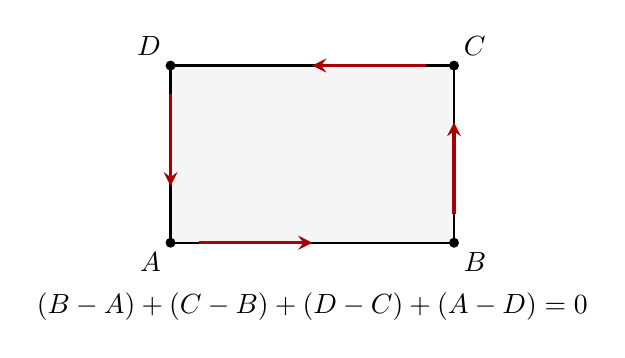
\begin{tikzpicture}[scale=0.9, >=stealth]
    \coordinate (A) at (0,0);
    \coordinate (B) at (4,0);
    \coordinate (C) at (4,2.5);
    \coordinate (D) at (0,2.5);

    \draw[fill=gray!8, thick] (A)--(B)--(C)--(D)--cycle;

    \draw[->, very thick, red!65!black] (0.4,0) -- (2.0,0);
    \draw[->, very thick, red!65!black] (4,0.4) -- (4,1.7);
    \draw[->, very thick, red!65!black] (3.6,2.5) -- (2.0,2.5);
    \draw[->, very thick, red!65!black] (0,2.1) -- (0,0.8);

    \fill (A) circle (2pt);
    \fill (B) circle (2pt);
    \fill (C) circle (2pt);
    \fill (D) circle (2pt);

    \node[below left] at (A) {\(A\)};
    \node[below right] at (B) {\(B\)};
    \node[above right] at (C) {\(C\)};
    \node[above left] at (D) {\(D\)};

    \node at (2,-0.9)
        {\((B-A)+(C-B)+(D-C)+(A-D)=0\)};
\end{tikzpicture}
\caption{The boundary of a rectangle is a closed curve.  Its boundary cancels at the
corners.}
\end{figure}

For a solid box, the same cancellation happens one dimension higher.  The boundary of
the box is made of faces.  The boundary of those faces is made of edges.  Every edge
belongs to two neighboring faces, and the two induced orientations are opposite.
So all edges cancel.

This explains why \(d^2=0\) belongs with Stokes-type theorems.  The general pattern is
\[
    \int_{\partial M}\alpha=\int_M d\alpha.
\]
Apply the same idea one more time:
\[
    \int_{\partial(\partial M)}\alpha
    =
    \int_{\partial M}d\alpha
    =
    \int_M d(d\alpha).
\]
The left side is zero because
\[
    \partial(\partial M)=0.
\]
The right side is zero because
\[
    d(d\alpha)=0.
\]

So the algebra and the geometry say the same thing:

\[
\boxed{
\begin{array}{c}
\text{algebra: } d^2=0,\\[1mm]
\text{geometry: } \partial^2=0.
\end{array}
}
\]

That is a small sentence with a large reach.  It says every exact form has zero exterior
derivative:
\[
    \alpha=d\beta
    \quad\Longrightarrow\quad
    d\alpha=0.
\]
But it does not answer the reverse question.  If a form has zero exterior derivative,
must it come from another form?  On a region with no holes, often yes.  Around a
missing point or a missing axis, sometimes no.  The next names are short, but they
open the door to the topology hiding inside vector calculus: \emph{closed} and
\emph{exact}.
\section{Closed and exact forms}
\label{sec:17.5}

Section \ref{sec:17.4} ended with the identity
\[
    d^2=0.
\]
That identity gives one direction for free:
\[
    \text{if a form is already a derivative, then its next derivative is zero.}
\]
The reverse question is more delicate.  If a form has zero exterior derivative, did it
come from another form?  Sometimes yes.  Sometimes a hole in the domain stops it.

\subsection{Exact forms: \texorpdfstring{\(\omega=d\alpha\)}{omega = d alpha}}

Start with a form whose origin is visible.

Let
\[
    \phi(x,y,z)=xz+y^2.
\]
Then
\[
    d\phi=z\,dx+2y\,dy+x\,dz.
\]
The \(1\)-form
\[
    \omega=z\,dx+2y\,dy+x\,dz
\]
is not just any \(1\)-form.  It is the exterior derivative of the \(0\)-form \(\phi\).

That gives it a special property.  Along any curve from \(A\) to \(B\),
\[
    \int_C \omega
    =
    \int_C d\phi
    =
    \phi(B)-\phi(A).
\]
The integral is an endpoint difference.  It does not remember the path.

This is the same exactness from Section \ref{sec:13.5}, now placed in the larger
forms ladder.

\begin{definition}[Exact form]
A \(k\)-form \(\alpha\) is called \emph{exact} on a domain \(D\) if there is a
\((k-1)\)-form \(\beta\) on \(D\) such that
\[
\boxed{
    \alpha=d\beta.
}
\]

For example:
\[
\begin{array}{c|c}
\text{Exact form} & \text{Means} \\ \hline
\omega=d\phi & \text{a \(1\)-form is the derivative of a function}\\[1mm]
\Phi=d\omega & \text{a \(2\)-form is the derivative of a \(1\)-form}\\[1mm]
\Theta=d\Phi & \text{a \(3\)-form is the derivative of a \(2\)-form}
\end{array}
\]
\end{definition}

The word \emph{exact} means that the form has a global antiderivative of the correct
degree.

Here are the three main degrees in ordinary space.

\begin{example}[An exact \(1\)-form]
Let
\[
    \phi(x,y,z)=xz+y^2.
\]
Then
\[
\boxed{
    d\phi=z\,dx+2y\,dy+x\,dz.
}
\]
So
\[
    z\,dx+2y\,dy+x\,dz
\]
is an exact \(1\)-form.
\end{example}

\begin{example}[An exact \(2\)-form]
Let
\[
    \omega=-y\,dx+x\,dy+z\,dz.
\]
Then
\[
\begin{aligned}
d\omega
&=
d(-y)\wedge dx+d(x)\wedge dy+d(z)\wedge dz\\
&=
(-dy)\wedge dx+dx\wedge dy+dz\wedge dz\\
&=
dx\wedge dy+dx\wedge dy+0\\
&=
2\,dx\wedge dy.
\end{aligned}
\]
Therefore
\[
\boxed{
    2\,dx\wedge dy=d(-y\,dx+x\,dy+z\,dz).
}
\]
So \(2\,dx\wedge dy\) is an exact \(2\)-form.
\end{example}

\begin{example}[An exact \(3\)-form]
The ordinary volume form is exact on \(\mathbb R^3\):
\[
\boxed{
    dx\wedge dy\wedge dz=d(x\,dy\wedge dz).
}
\]
Indeed,
\[
\begin{aligned}
d(x\,dy\wedge dz)
&=
dx\wedge dy\wedge dz.
\end{aligned}
\]
So even a \(3\)-form can be an exterior derivative.
\end{example}

Exactness is not only a formula.  It is a formula on a domain.  The antiderivative form
has to exist on the whole domain where we want to use it.

\subsection{Closed forms: \texorpdfstring{\(d\omega=0\)}{d omega = 0}}

Now forget where the form came from and ask only what happens when we apply \(d\).

For the exact \(1\)-form
\[
    \omega=z\,dx+2y\,dy+x\,dz=d(xz+y^2),
\]
we get
\[
    d\omega=d(d\phi)=0.
\]
For the exact \(2\)-form
\[
    \Phi=2\,dx\wedge dy=d(-y\,dx+x\,dy+z\,dz),
\]
we get
\[
    d\Phi=0.
\]
For the exact \(3\)-form
\[
    \Theta=dx\wedge dy\wedge dz=d(x\,dy\wedge dz),
\]
we also have
\[
    d\Theta=0,
\]
because every \(3\)-form in ordinary space has zero exterior derivative.

This property gets its own name.

\begin{definition}[Closed form]
A form \(\alpha\) is called \emph{closed} if
\[
\boxed{
    d\alpha=0.
}
\]
\end{definition}

Closed means that the next exterior derivative vanishes.

For \(1\)-forms in the plane,
\[
    \omega=P\,dx+Q\,dy
\]
is closed exactly when
\[
\boxed{
    Q_x-P_y=0.
}
\]
That is the scalar-curl test.

For \(1\)-forms in space,
\[
    \omega=P\,dx+Q\,dy+R\,dz
\]
is closed exactly when
\[
\boxed{
    \nabla\times(P,Q,R)=\mathbf 0.
}
\]

For flux \(2\)-forms in space,
\[
    \Phi=P\,dy\wedge dz+Q\,dz\wedge dx+R\,dx\wedge dy
\]
is closed exactly when
\[
\boxed{
    P_x+Q_y+R_z=0.
}
\]
In vector language, this says
\[
\boxed{
    \nabla\cdot(P,Q,R)=0.
}
\]

So the old vector-calculus words fit into one table:

\[
\begin{array}{c|c|c}
\text{Form} & \text{Closed condition} & \text{Vector-language translation} \\ \hline
P\,dx+Q\,dy & d\omega=0 & Q_x-P_y=0\\[1mm]
P\,dx+Q\,dy+R\,dz & d\omega=0 & \nabla\times(P,Q,R)=\mathbf 0\\[1mm]
P\,dy\wedge dz+Q\,dz\wedge dx+R\,dx\wedge dy & d\Phi=0 &
\nabla\cdot(P,Q,R)=0
\end{array}
\]

\subsection{Exact implies closed}

The identity
\[
    d^2=0
\]
is exactly the statement that every exact form is closed.

\begin{theorem}[Exact forms are closed]
Let \(\alpha\) be a form with smooth enough coefficients for the identity
\[
    d^2=0
\]
to apply.  If \(\alpha\) is exact, then \(\alpha\) is closed.

In symbols,
\[
\boxed{
    \alpha=d\beta
    \quad\Longrightarrow\quad
    d\alpha=0.
}
\]
\end{theorem}

\begin{proof}
If \(\alpha=d\beta\), then
\[
    d\alpha=d(d\beta)=d^2\beta=0.
\]
So \(\alpha\) is closed.
\end{proof}

This theorem contains a smoothness phrase for a reason.  The cancellation in
\[
    d^2=0
\]
uses equality of mixed partial derivatives.  Section \ref{sec:17.4} showed a function
\[
    g(x,y)=
    \begin{cases}
    \dfrac{xy(x^2-y^2)}{x^2+y^2}, & (x,y)\ne(0,0),\\[2mm]
    0, & (x,y)=(0,0),
    \end{cases}
\]
for which
\[
    g_{xy}(0,0)=-1,
    \qquad
    g_{yx}(0,0)=1.
\]
If we try to use the smooth-form rule at the origin without the smoothness, the usual
cancellation fails.  The identity \(d^2=0\) is a theorem for smooth forms, not a license
to ignore broken mixed partials.

\subsection{Closed does not always imply exact}

The reverse statement is the tempting one:
\[
    d\alpha=0
    \quad\stackrel{?}{\Longrightarrow}\quad
    \alpha=d\beta.
\]
It is false on domains with holes.

The cleanest example is the angle form
\[
    \alpha=
    \frac{-y}{x^2+y^2}\,dx+
    \frac{x}{x^2+y^2}\,dy
\]
on the punctured plane
\[
    D=\mathbb R^2\setminus\{(0,0)\}.
\]
The origin is missing, so the formula is defined everywhere on \(D\).

Let
\[
    P=\frac{-y}{x^2+y^2},
    \qquad
    Q=\frac{x}{x^2+y^2}.
\]
Then
\[
\begin{aligned}
P_y
&=
\frac{y^2-x^2}{(x^2+y^2)^2},
\end{aligned}
\]
and
\[
\begin{aligned}
Q_x
&=
\frac{y^2-x^2}{(x^2+y^2)^2}.
\end{aligned}
\]
So
\[
    Q_x-P_y=0,
\]
and therefore
\[
\boxed{
    d\alpha=0
}
\]
on the punctured plane.  The form is closed.

Now integrate around the unit circle
\[
    C:\quad \mathbf r(t)=(\cos t,\sin t),
    \qquad 0\le t\le2\pi.
\]
Along \(C\),
\[
    dx=-\sin t\,dt,
    \qquad
    dy=\cos t\,dt,
\]
and
\[
    x^2+y^2=1.
\]
Thus
\[
\begin{aligned}
\mathbf r^*\alpha
&=
-\sin t(-\sin t\,dt)+\cos t(\cos t\,dt)\\
&=
dt.
\end{aligned}
\]
So
\[
\boxed{
    \oint_C\alpha=2\pi.
}
\]

If \(\alpha\) were exact on \(D\), then
\[
    \alpha=d\theta
\]
for some single-valued function \(\theta\) on all of \(D\).  The fundamental theorem for
line integrals would give
\[
    \oint_C d\theta=0,
\]
because \(C\) starts and ends at the same point.

But the integral is \(2\pi\).  Therefore
\[
\boxed{
    \alpha \text{ is closed but not exact on } \mathbb R^2\setminus\{(0,0)\}.
}
\]

\begin{figure}[h]
\centering
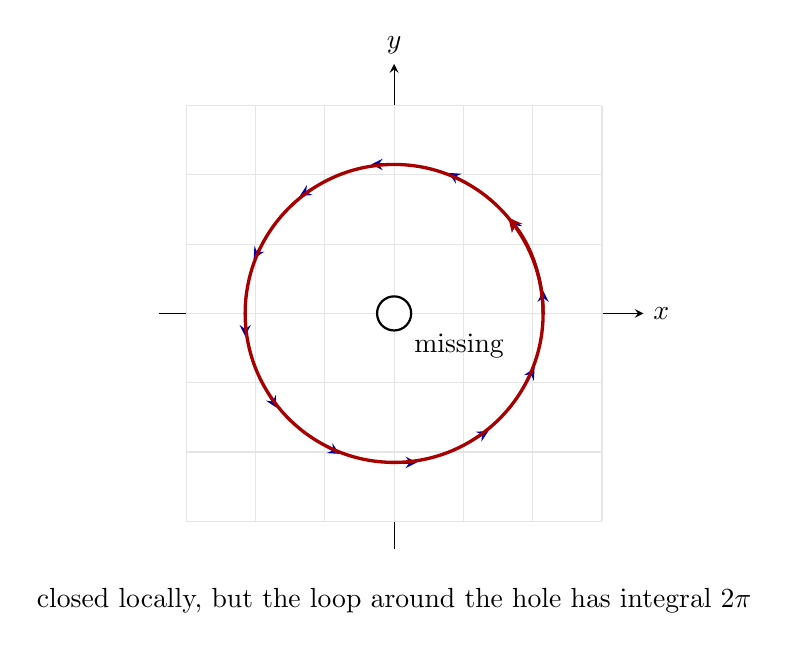
\begin{tikzpicture}[scale=0.88, >=stealth]
    \draw[->] (-3.4,0) -- (3.6,0) node[right] {\(x\)};
    \draw[->] (0,-3.4) -- (0,3.6) node[above] {\(y\)};

    \draw[gray!20, step=1] (-3,-3) grid (3,3);

    \foreach \a in {0,30,...,330} {
        \pgfmathsetmacro{\x}{2.15*cos(\a)}
        \pgfmathsetmacro{\y}{2.15*sin(\a)}
        \draw[->, blue!65!black, thick]
            (\x,\y) -- ++({-0.33*sin(\a)},{0.33*cos(\a)});
    }

    \draw[very thick, red!65!black] (0,0) circle (2.15);
    \draw[->, very thick, red!65!black] (2.15,0) arc[start angle=0,end angle=40,radius=2.15];

    \fill[white] (0,0) circle (7pt);
    \draw[thick] (0,0) circle (7pt);
    \node[below right] at (0.15,-0.15) {missing};

    \node at (0,-4.15)
        {closed locally, but the loop around the hole has integral \(2\pi\)};
\end{tikzpicture}
\caption{A closed \(1\)-form can fail to be exact when the domain has a hole.}
\end{figure}

This is the first place where topology enters the story.  The formula
\[
    d\alpha=0
\]
is local.  It checks tiny rectangles.  Exactness is global.  It asks whether one
potential works on the whole domain.

\subsection{Holes, topology, and conservative fields}

For \(1\)-forms, the old conservative-field language now becomes a special case of the
closed-exact language.

Let
\[
    \omega=P\,dx+Q\,dy+R\,dz
\]
be the work form of a vector field
\[
    \mathbf F=(P,Q,R).
\]

Then
\[
\begin{array}{c|c|c}
\text{Forms language} & \text{Vector language} & \text{Meaning} \\ \hline
\omega=d\phi & \mathbf F=\nabla\phi &
\text{conservative field}\\[1mm]
d\omega=0 & \nabla\times\mathbf F=\mathbf 0 &
\text{curl-free field}\\[1mm]
\displaystyle \oint_C\omega=0\text{ for all closed }C
& \text{zero work around every closed loop}
& \text{path independence}
\end{array}
\]

On the simple domains from ordinary calculus, such as rectangles, disks, boxes, and
balls, a smooth closed \(1\)-form is exact.  In vector language:
\[
\boxed{
    \text{curl-free on a no-hole domain}
    \quad\Longrightarrow\quad
    \text{conservative.}
}
\]
But if the domain has a hole, the implication can fail:
\[
\boxed{
    \text{closed}
    \not\Longrightarrow
    \text{exact}.
}
\]

The angle form \(\alpha\) is the model example.  Away from the origin it has no local
curl.  But a loop around the missing origin measures \(2\pi\).  The hole is invisible to
\(d\alpha\), but visible to integration.

That sentence is the main point:

\[
\boxed{
    d\alpha=0 \text{ is local; } \alpha=d\beta \text{ is global.}
}
\]

The same issue can happen one degree higher.  A closed flux \(2\)-form can have zero
divergence everywhere it is defined and still fail to be the exterior derivative of a
global \(1\)-form.  In the next warning examples, a loop around a missing point and a
sphere around a missing point will both detect information that the local derivative
cannot see.

\section{Warning examples}
\label{sec:17.6}

The words \emph{closed} and \emph{exact} are short, but they hide the most common
mistake in vector calculus: checking a derivative and forgetting the domain.

A derivative sees what happens near each point.  An integral can walk around a hole.
Those are different powers.

\subsection{A closed \texorpdfstring{\(1\)}{1}-form on a punctured plane that is not exact}

Return to the punctured plane
\[
    D=\mathbb R^2\setminus\{(0,0)\}
\]
and the \(1\)-form
\[
\boxed{
    \alpha=
    \frac{-y}{x^2+y^2}\,dx+
    \frac{x}{x^2+y^2}\,dy.
}
\]

We already computed
\[
    d\alpha=0
\]
on \(D\).  So \(\alpha\) is closed.

But around the unit circle,
\[
    C:\quad \mathbf r(t)=(\cos t,\sin t),
    \qquad 0\le t\le2\pi,
\]
we get
\[
    \mathbf r^*\alpha=dt.
\]
Hence
\[
\boxed{
    \oint_C\alpha=2\pi.
}
\]

This one number proves that \(\alpha\) is not exact on \(D\).  If
\[
    \alpha=d\theta
\]
on all of \(D\), then the integral around every closed curve would be zero:
\[
    \oint_C d\theta=\theta(C_{\text{end}})-\theta(C_{\text{start}})=0.
\]
But \(C_{\text{end}}=C_{\text{start}}\), and the integral is \(2\pi\).

So the form satisfies
\[
    d\alpha=0
\]
but fails
\[
    \alpha=d\theta
\]
globally.

The missing point matters.  The loop cannot shrink to a point without crossing the
place where the form is not defined.

\subsection{A locally exact form with a global obstruction}

The same form
\[
    \alpha=
    \frac{-y}{x^2+y^2}\,dx+
    \frac{x}{x^2+y^2}\,dy
\]
really is an angle differential locally.

On the right half-plane
\[
    D_+=\{(x,y):x>0\},
\]
define
\[
    \theta(x,y)=\arctan\left(\frac{y}{x}\right).
\]
Then
\[
\begin{aligned}
\theta_x
&=
\frac{1}{1+(y/x)^2}\left(-\frac{y}{x^2}\right)\\
&=
\frac{x^2}{x^2+y^2}\left(-\frac{y}{x^2}\right)\\
&=
\frac{-y}{x^2+y^2},
\end{aligned}
\]
and
\[
\begin{aligned}
\theta_y
&=
\frac{1}{1+(y/x)^2}\left(\frac1x\right)\\
&=
\frac{x^2}{x^2+y^2}\left(\frac1x\right)\\
&=
\frac{x}{x^2+y^2}.
\end{aligned}
\]
Therefore
\[
\boxed{
    d\theta=\alpha
}
\]
on \(D_+\).

So \(\alpha\) is exact on the right half-plane.

The problem is not local.  Near any point of the punctured plane, we can choose a
small neighborhood and a continuous angle function there.  On that small neighborhood,
\[
    \alpha=d\theta.
\]
The problem is global.  No single continuous angle function can be chosen on the whole
punctured plane.

Here is the obstruction in one line.  Suppose there were a global function \(\theta\) on
\(D\) with
\[
    d\theta=\alpha.
\]
Along the unit circle,
\[
    \frac{d}{dt}\theta(\cos t,\sin t)
    =
    \mathbf r^*(d\theta)
    =
    \mathbf r^*\alpha
    =
    1.
\]
So
\[
    \theta(\cos t,\sin t)=t+C.
\]
At \(t=0\) and \(t=2\pi\), the point on the circle is the same:
\[
    (1,0).
\]
But the formula would give values differing by \(2\pi\):
\[
    C
    \qquad\text{and}\qquad
    2\pi+C.
\]
A single-valued function cannot do that.

\begin{figure}[h]
\centering
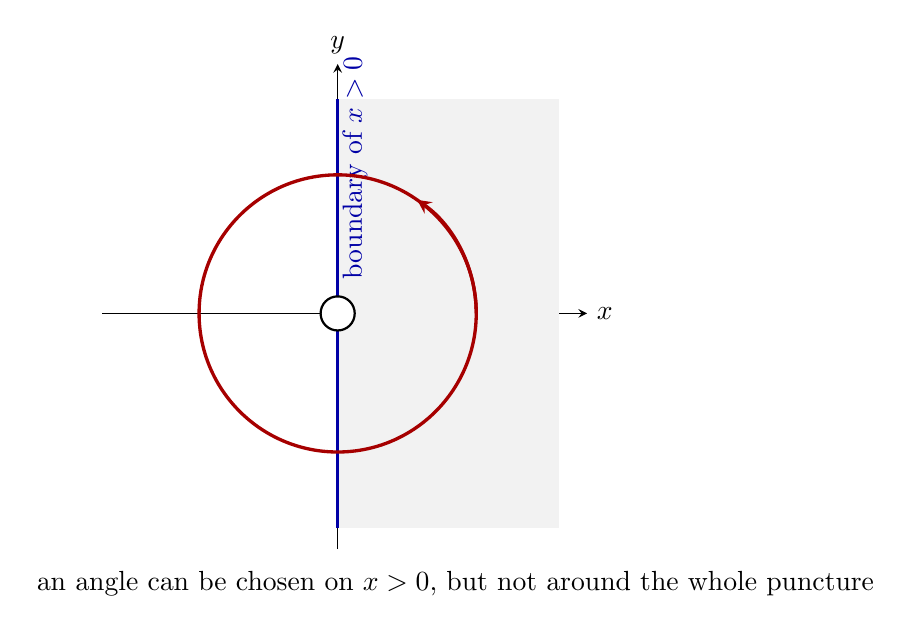
\begin{tikzpicture}[scale=0.88, >=stealth]
    \draw[->] (-3.4,0) -- (3.6,0) node[right] {\(x\)};
    \draw[->] (0,-3.4) -- (0,3.6) node[above] {\(y\)};

    \fill[gray!10] (0,-3.1) rectangle (3.2,3.1);
    \draw[very thick, blue!65!black] (0,-3.1) -- (0,3.1);
    \node[blue!65!black, rotate=90] at (0.25,2.1) {boundary of \(x>0\)};

    \draw[very thick, red!65!black] (0,0) circle (2.0);
    \draw[->, very thick, red!65!black] (2.0,0) arc[start angle=0,end angle=55,radius=2.0];

    \fill[white] (0,0) circle (7pt);
    \draw[thick] (0,0) circle (7pt);

    \node at (1.7,-3.9)
        {an angle can be chosen on \(x>0\), but not around the whole puncture};
\end{tikzpicture}
\caption{The angle function works on a half-plane.  It cannot be made single-valued
around a full loop.}
\end{figure}

This is the difference between local and global exactness:

\[
\boxed{
\begin{array}{c}
\text{locally exact: potentials exist in small neighborhoods},\\[1mm]
\text{globally exact: one potential works on the whole domain.}
\end{array}
}
\]

A hole can prevent local potentials from gluing into one global potential.

\subsection{A singular form that breaks the theorem if the singularity is ignored}

The same warning appears in space, one degree higher.

Let
\[
    r=\sqrt{x^2+y^2+z^2},
\]
and define the vector field
\[
    \mathbf G(x,y,z)=\frac{(x,y,z)}{r^3}
\]
on
\[
    \mathbb R^3\setminus\{(0,0,0)\}.
\]
Its flux \(2\)-form is
\[
\boxed{
    \Phi=
    \frac{x}{r^3}\,dy\wedge dz+
    \frac{y}{r^3}\,dz\wedge dx+
    \frac{z}{r^3}\,dx\wedge dy.
}
\]

Away from the origin,
\[
    d\Phi=(\nabla\cdot\mathbf G)\,dx\wedge dy\wedge dz.
\]
Compute the divergence.  Since
\[
    \frac{\partial}{\partial x}\left(\frac{x}{r^3}\right)
    =
    \frac1{r^3}-\frac{3x^2}{r^5},
\]
and similarly for \(y\) and \(z\),
\[
\begin{aligned}
\nabla\cdot\mathbf G
&=
\left(\frac1{r^3}-\frac{3x^2}{r^5}\right)
+
\left(\frac1{r^3}-\frac{3y^2}{r^5}\right)
+
\left(\frac1{r^3}-\frac{3z^2}{r^5}\right)\\
&=
\frac3{r^3}-\frac{3(x^2+y^2+z^2)}{r^5}\\
&=
\frac3{r^3}-\frac{3r^2}{r^5}\\
&=
0.
\end{aligned}
\]
Thus
\[
\boxed{
    d\Phi=0
}
\]
wherever \(\Phi\) is defined.

Now integrate over the sphere \(S_a\) of radius \(a\), oriented outward.  On that
sphere,
\[
    \widehat{\mathbf n}=\frac{(x,y,z)}{a},
\]
and
\[
    \mathbf G=\frac{(x,y,z)}{a^3}.
\]
Therefore
\[
    \mathbf G\cdot\widehat{\mathbf n}
    =
    \frac{x^2+y^2+z^2}{a^4}
    =
    \frac{a^2}{a^4}
    =
    \frac1{a^2}.
\]
So
\[
\boxed{
    \int_{S_a}\Phi
    =
    \iint_{S_a}\mathbf G\cdot\widehat{\mathbf n}\,dS
    =
    \frac1{a^2}\cdot 4\pi a^2
    =
    4\pi.
}
\]

It is tempting to say:
\[
    d\Phi=0,
    \qquad
    \text{so the flux through the sphere should be }0.
\]
That is the mistake.  The form is not defined at the origin, and the origin lies inside
the sphere.

The divergence theorem cannot be applied to the whole ball
\[
    x^2+y^2+z^2\le a^2,
\]
because \(\Phi\) is not smooth on that ball.  It is not even defined at the center.

If we remove a small ball around the origin, the theorem works perfectly.  Let
\[
    E_{\varepsilon,a}
    =
    \{(x,y,z):\varepsilon\le r\le a\}.
\]
This is a spherical shell.  Its boundary has two pieces:
\[
    \partial E_{\varepsilon,a}=S_a- S_\varepsilon.
\]
The minus sign appears because the outward normal for the shell on the inner sphere
points toward the origin.

Since
\[
    d\Phi=0
\]
on the shell,
\[
    \int_{\partial E_{\varepsilon,a}}\Phi
    =
    \int_{E_{\varepsilon,a}}d\Phi
    =
    0.
\]
And indeed,
\[
    \int_{S_a}\Phi-\int_{S_\varepsilon}\Phi
    =
    4\pi-4\pi
    =
    0.
\]

The singularity is not a minor defect.  It carries the missing flux.

\begin{figure}[h]
\centering
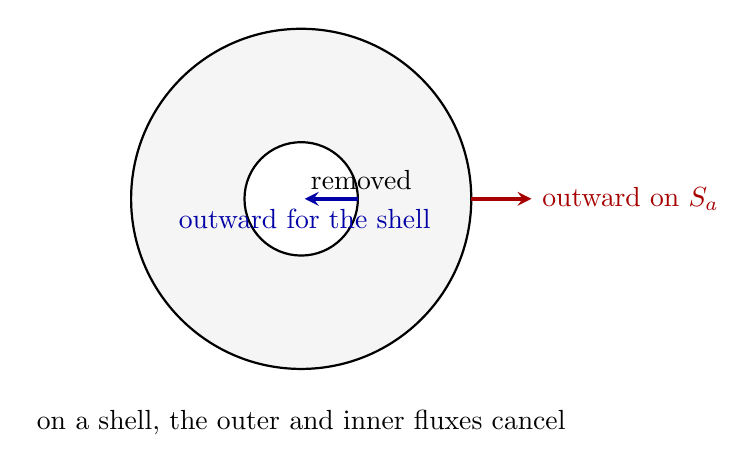
\begin{tikzpicture}[scale=0.9, >=stealth]
    \draw[fill=gray!8, thick] (0,0) circle (2.4);
    \draw[fill=white, thick] (0,0) circle (0.8);

    \draw[->, very thick, red!65!black] (2.4,0) -- (3.25,0)
        node[right] {outward on \(S_a\)};
    \draw[->, very thick, blue!65!black] (0.8,0) -- (0.05,0)
        node[below] {outward for the shell};

    \node [above right] at (0,0) {removed};
    \node at (0,-3.15)
        {on a shell, the outer and inner fluxes cancel};
\end{tikzpicture}
\caption{Removing the singular point turns the ball into a shell.  The boundary now has
two spheres with opposite induced orientations.}
\end{figure}

\subsection{Why ``zero derivative'' can hide global information}

The two examples have the same shape.

In the punctured plane,
\[
    \alpha=
    \frac{-y}{x^2+y^2}\,dx+
    \frac{x}{x^2+y^2}\,dy
\]
satisfies
\[
    d\alpha=0,
\]
but
\[
    \int_{\text{unit circle}}\alpha=2\pi.
\]

In punctured space,
\[
    \Phi=
    \frac{x}{r^3}\,dy\wedge dz+
    \frac{y}{r^3}\,dz\wedge dx+
    \frac{z}{r^3}\,dx\wedge dy
\]
satisfies
\[
    d\Phi=0,
\]
but
\[
    \int_{\text{unit sphere}}\Phi=4\pi.
\]

Put side by side:

\[
\begin{array}{c|c|c|c}
\text{Domain} & \text{Closed form} & \text{Closed object} & \text{Integral} \\ \hline
\mathbb R^2\setminus\{0\}
&
\displaystyle
\frac{-y\,dx+x\,dy}{x^2+y^2}
&
\text{circle around the missing point}
&
2\pi
\\[4mm]
\mathbb R^3\setminus\{0\}
&
\displaystyle
\frac{x}{r^3}\,dy\wedge dz+
\frac{y}{r^3}\,dz\wedge dx+
\frac{z}{r^3}\,dx\wedge dy
&
\text{sphere around the missing point}
&
4\pi
\end{array}
\]

The word \emph{closed} has two meanings in this discussion, and both matter.

A form is closed when
\[
    d\alpha=0.
\]
A curve or surface is closed when it has no boundary:
\[
    \partial C=0,
    \qquad
    \partial S=0.
\]

If a form is exact, then its integral over a closed object must vanish.  For a closed
curve,
\[
    \int_C d\phi=0.
\]
For a closed surface,
\[
    \int_S d\omega=0.
\]
The boundary of the boundary has nothing left to measure.

So a nonzero integral over a closed loop or closed surface is a certificate:
\[
\boxed{
    \text{the form is not exact on that domain.}
}
\]

The derivative \(d\) checks local density: local curl, local source, local change.  A
closed loop or surface can check something larger: whether the domain has a missing
piece that the form winds around.

That is why the next theorem has to mention both objects:
\[
    \text{a form}
    \qquad\text{and}\qquad
    \text{the boundary of the region where it is integrated.}
\]
The next section will put the whole chapter into one translation table.  Then Chapter
\ref{ch:18} gives the single boundary theorem that explains why all these local and
global pieces fit together:
\[
    \int_{\partial M}\omega=\int_M d\omega.
\]
\section{Chapter review and translation table}
\label{sec:17.7}

Section \ref{sec:17.6} ended with a warning.  The equation
\[
    d\alpha=0
\]
is local.  It checks what happens near each point where the form is defined.  But
integrals around closed loops and closed surfaces can detect something larger:
a missing point, a missing axis, or a hole in the domain.

Now we collect the whole chapter into one dictionary.

The exterior derivative does one simple thing:

\[
\boxed{
    d \text{ raises degree by }1.
}
\]

In ordinary three-dimensional space, the ladder is
\[
    0\text{-forms}
    \xrightarrow{\ d\ }
    1\text{-forms}
    \xrightarrow{\ d\ }
    2\text{-forms}
    \xrightarrow{\ d\ }
    3\text{-forms}
    \xrightarrow{\ d\ }
    0.
\]
The last arrow gives zero because there are no nonzero \(4\)-forms in ordinary
three-dimensional space.

The practical rule is just as simple:

\[
\boxed{
    \text{Differentiate the coefficient, then wedge with the coordinate factors.}
}
\]

The wedge product then takes care of the signs:
\[
    dx\wedge dx=0,
    \qquad
    dx\wedge dy=-dy\wedge dx.
\]

\subsection{\texorpdfstring{\(d\)}{d} on \texorpdfstring{\(0\)}{0}-forms:
gradient information}

A \(0\)-form is a function.  Its exterior derivative is the differential.

If
\[
    f=f(x,y,z),
\]
then
\[
\boxed{
    df=f_x\,dx+f_y\,dy+f_z\,dz.
}
\]
This \(1\)-form measures tangent vectors:
\[
    df_{\mathbf p}(\mathbf v)
    =
    f_x(\mathbf p)v_x+f_y(\mathbf p)v_y+f_z(\mathbf p)v_z.
\]

The gradient is the vector that represents this same measurement when we use the
Euclidean dot product:
\[
\boxed{
    df_{\mathbf p}(\mathbf v)
    =
    \nabla f(\mathbf p)\cdot \mathbf v.
}
\]

\begin{example}[A \(0\)-form and its first-order change]
Let
\[
    f(x,y,z)=x^2y+yz.
\]
Then
\[
    f_x=2xy,
    \qquad
    f_y=x^2+z,
    \qquad
    f_z=y.
\]
So
\[
\boxed{
    df=2xy\,dx+(x^2+z)\,dy+y\,dz.
}
\]

At the point
\[
    P=(1,2,3),
\]
this becomes
\[
    df_P=4\,dx+4\,dy+2\,dz.
\]
If a particle passes through \(P\) with velocity
\[
    \mathbf v=(2,-1,3),
\]
then
\[
\begin{aligned}
    df_P(\mathbf v)
    &=
    4(2)+4(-1)+2(3)\\
    &=
    10.
\end{aligned}
\]
So \(f\) is increasing at rate \(10\) along that motion.

In gradient notation,
\[
    \nabla f(P)=(4,4,2),
\]
and
\[
    \nabla f(P)\cdot \mathbf v
    =
    (4,4,2)\cdot(2,-1,3)
    =
    10.
\]
\end{example}

So the first row of the dictionary is:

\[
\boxed{
    \text{exterior derivative of a function}
    =
    \text{gradient information as a \(1\)-form}.
}
\]

But \(df\) is not mainly a vector.  It is a covector, a measuring rule for tangent
vectors.  The gradient vector appears only after the dot product translates that
measuring rule into a vector.

\subsection{\texorpdfstring{\(d\)}{d} on \texorpdfstring{\(1\)}{1}-forms:
curl information}

A \(1\)-form is integrated along curves.  Its exterior derivative is a \(2\)-form, so it is
integrated over surfaces.  This is why \(d\omega\) measures circulation density.

In the plane, let
\[
    \omega=P\,dx+Q\,dy.
\]
Then
\[
\boxed{
    d\omega=(Q_x-P_y)\,dx\wedge dy.
}
\]
The coefficient
\[
    Q_x-P_y
\]
is the scalar curl in the plane.

So Green's theorem can be read as
\[
    \text{circulation around the boundary}
    =
    \text{circulation density added over the inside}.
\]

In space, let
\[
    \omega=P\,dx+Q\,dy+R\,dz.
\]
Then
\[
\boxed{
    d\omega
    =
    (R_y-Q_z)\,dy\wedge dz
    +
    (P_z-R_x)\,dz\wedge dx
    +
    (Q_x-P_y)\,dx\wedge dy.
}
\]

If
\[
    \mathbf F=(P,Q,R)
\]
and
\[
    \omega_{\mathbf F}=P\,dx+Q\,dy+R\,dz,
\]
then
\[
\boxed{
    d\omega_{\mathbf F}=\Phi_{\nabla\times\mathbf F}.
}
\]
In words:

\[
\boxed{
    \text{the exterior derivative of a work form is the curl as a flux form.}
}
\]

\begin{example}[A \(1\)-form and its curl \(2\)-form]
Let
\[
    \omega=(xy+z)\,dx+(y^2+xz)\,dy+(x^2-y)\,dz.
\]
Here
\[
    P=xy+z,
    \qquad
    Q=y^2+xz,
    \qquad
    R=x^2-y.
\]
Compute the three curl coefficients:
\[
    R_y-Q_z=-1-x,
\]
\[
    P_z-R_x=1-2x,
\]
and
\[
    Q_x-P_y=z-x.
\]
Therefore
\[
\boxed{
    d\omega
    =
    (-1-x)\,dy\wedge dz
    +
    (1-2x)\,dz\wedge dx
    +
    (z-x)\,dx\wedge dy.
}
\]

If
\[
    \mathbf F=(xy+z,\ y^2+xz,\ x^2-y),
\]
then
\[
    \nabla\times\mathbf F=(-1-x,\ 1-2x,\ z-x),
\]
and \(d\omega\) is exactly the flux form of that curl.
\end{example}

The standard order
\[
    dy\wedge dz,\qquad dz\wedge dx,\qquad dx\wedge dy
\]
is not accidental.  These are the three coordinate area forms perpendicular to the
\(x\)-, \(y\)-, and \(z\)-axes:

\[
\begin{array}{c|c|c}
\text{Area form} & \text{Measures oriented shadow in} & \text{Matches component} \\ \hline
dy\wedge dz & yz\text{-plane} & x\text{-component}\\[1mm]
dz\wedge dx & zx\text{-plane} & y\text{-component}\\[1mm]
dx\wedge dy & xy\text{-plane} & z\text{-component}
\end{array}
\]

That is why the curl vector becomes a flux \(2\)-form in exactly this order.

\subsection{\texorpdfstring{\(d\)}{d} on \texorpdfstring{\(2\)}{2}-forms:
divergence information}

A \(2\)-form is integrated over surfaces.  Its exterior derivative is a \(3\)-form, so it
is integrated over solids.  This is why \(d\Phi\) measures source density.

In space, a flux \(2\)-form has the shape
\[
    \Phi
    =
    P\,dy\wedge dz
    +
    Q\,dz\wedge dx
    +
    R\,dx\wedge dy.
\]
Then
\[
\boxed{
    d\Phi
    =
    (P_x+Q_y+R_z)\,dx\wedge dy\wedge dz.
}
\]

If
\[
    \mathbf F=(P,Q,R),
\]
then
\[
    P_x+Q_y+R_z=\nabla\cdot\mathbf F.
\]
So
\[
\boxed{
    d\Phi_{\mathbf F}
    =
    (\nabla\cdot\mathbf F)\,dx\wedge dy\wedge dz.
}
\]

In words:

\[
\boxed{
    \text{the exterior derivative of a flux form is divergence as a volume form.}
}
\]

\begin{example}[A \(2\)-form and its source density]
Let
\[
    \Phi
    =
    (x^2+yz)\,dy\wedge dz
    +
    (\sin y+xz)\,dz\wedge dx
    +
    (xy+e^z)\,dx\wedge dy.
\]
Here
\[
    P=x^2+yz,
    \qquad
    Q=\sin y+xz,
    \qquad
    R=xy+e^z.
\]
Therefore
\[
    P_x=2x,
    \qquad
    Q_y=\cos y,
    \qquad
    R_z=e^z.
\]
So
\[
\boxed{
    d\Phi=(2x+\cos y+e^z)\,dx\wedge dy\wedge dz.
}
\]
The coefficient
\[
    2x+\cos y+e^z
\]
is the divergence of the vector field whose flux form is \(\Phi\).
\end{example}

This is the third row of the dictionary:

\[
\boxed{
    \text{exterior derivative of a flux form}
    =
    \text{divergence information as a volume form}.
}
\]

\subsection*{The two forms attached to a vector field}

A vector field in space can be turned into two different forms.  They do different
jobs.

If
\[
    \mathbf F=(P,Q,R),
\]
then its \emph{work form} is
\[
\boxed{
    \omega_{\mathbf F}=P\,dx+Q\,dy+R\,dz.
}
\]
This is integrated over curves.

Its \emph{flux form} is
\[
\boxed{
    \Phi_{\mathbf F}
    =
    P\,dy\wedge dz
    +
    Q\,dz\wedge dx
    +
    R\,dx\wedge dy.
}
\]
This is integrated over surfaces.

The exterior derivative treats these two forms differently:

\[
\begin{array}{c|c|c|c}
\text{Vector field used as} & \text{Form} & \text{Integrated over} & \text{Exterior derivative} \\ \hline
\text{work field} &
\omega_{\mathbf F}=P\,dx+Q\,dy+R\,dz &
\text{curves} &
d\omega_{\mathbf F}=\Phi_{\nabla\times\mathbf F}
\\[2mm]
\text{flux field} &
\Phi_{\mathbf F}=P\,dy\wedge dz+Q\,dz\wedge dx+R\,dx\wedge dy &
\text{surfaces} &
d\Phi_{\mathbf F}=(\nabla\cdot\mathbf F)\,dx\wedge dy\wedge dz
\end{array}
\]

This is a common place to mix things up.  The same vector field
\[
    \mathbf F=(P,Q,R)
\]
does not automatically tell us whether we are doing work or flux.  The form tells us.

\subsection*{The whole dictionary}

The chapter can now be compressed into one table.

\[
\begin{array}{c|c|c|c}
\text{Degree} & \text{Typical form in }\mathbb R^3
& \text{Integrated over} & d\text{ gives} \\ \hline
0 &
f &
\text{oriented points} &
df=f_x\,dx+f_y\,dy+f_z\,dz
\\[2mm]
1 &
P\,dx+Q\,dy+R\,dz &
\text{curves} &
\text{curl as a }2\text{-form}
\\[2mm]
2 &
P\,dy\wedge dz+Q\,dz\wedge dx+R\,dx\wedge dy &
\text{surfaces} &
\text{divergence as a }3\text{-form}
\\[2mm]
3 &
H\,dx\wedge dy\wedge dz &
\text{solids} &
0
\end{array}
\]

The classical vector-calculus names are shadows of the same operation:

\[
\boxed{
\begin{array}{ccl}
f & \xrightarrow{\ d\ } & df
\quad\text{contains gradient information},\\[1mm]
\omega_{\mathbf F} & \xrightarrow{\ d\ } & \Phi_{\nabla\times\mathbf F}
\quad\text{contains curl information},\\[1mm]
\Phi_{\mathbf F} & \xrightarrow{\ d\ } &
(\nabla\cdot\mathbf F)\,dx\wedge dy\wedge dz
\quad\text{contains divergence information}.
\end{array}
}
\]

\begin{figure}[h]
\centering
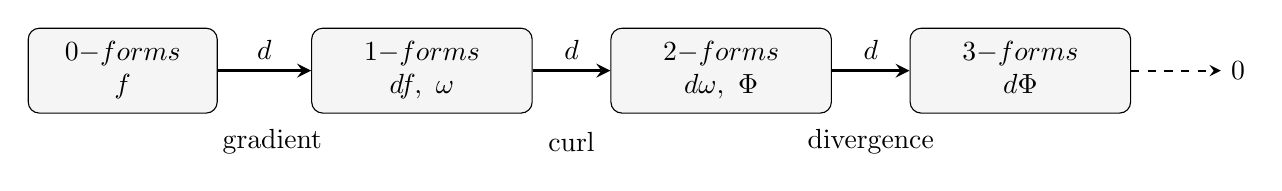
\begin{tikzpicture}[>=stealth, scale=0.95]
    \node[draw, rounded corners, fill=gray!8, minimum width=2.4cm, minimum height=1cm] (A)
        at (0,0) {\(\begin{array}{c}0\text{-forms}\\ f\end{array}\)};
    \node[draw, rounded corners, fill=gray!8, minimum width=2.8cm, minimum height=1cm] (B)
        at (4,0) {\(\begin{array}{c}1\text{-forms}\\ df,\ \omega\end{array}\)};
    \node[draw, rounded corners, fill=gray!8, minimum width=2.8cm, minimum height=1cm] (C)
        at (8,0) {\(\begin{array}{c}2\text{-forms}\\ d\omega,\ \Phi\end{array}\)};
    \node[draw, rounded corners, fill=gray!8, minimum width=2.8cm, minimum height=1cm] (D)
        at (12,0) {\(\begin{array}{c}3\text{-forms}\\ d\Phi\end{array}\)};

    \draw[->, very thick] (A) -- (B) node[midway, above] {\(d\)};
    \draw[->, very thick] (B) -- (C) node[midway, above] {\(d\)};
    \draw[->, very thick] (C) -- (D) node[midway, above] {\(d\)};

    \node at (2,-0.95) {gradient};
    \node at (6,-0.95) {curl};
    \node at (10,-0.95) {divergence};

    \draw[->, thick, dashed] (D.east) -- ++(1.2,0) node[right] {\(0\)};
\end{tikzpicture}
\caption{Gradient, curl, and divergence are one operation, \(d\), seen in different
degrees.}
\end{figure}

\subsection*{Closed, exact, and the role of holes}

The identity
\[
\boxed{
    d^2=0
}
\]
says that every exact form is closed:
\[
    \alpha=d\beta
    \quad\Longrightarrow\quad
    d\alpha=0.
\]

In vector language, this gives the familiar identities:
\[
\boxed{
    \nabla\times(\nabla f)=\mathbf 0
}
\]
and
\[
\boxed{
    \nabla\cdot(\nabla\times\mathbf F)=0.
}
\]

In forms language, both are the same statement:
\[
    d(d(\text{something}))=0.
\]

The reverse direction is the delicate one.

\[
\begin{array}{c|c|c}
\text{Word} & \text{Meaning} & \text{Warning} \\ \hline
\text{exact} & \alpha=d\beta & \text{automatically closed}\\[1mm]
\text{closed} & d\alpha=0 & \text{not always exact}\\[1mm]
\text{closed but not exact} & d\alpha=0,\ \alpha\ne d\beta
& \text{usually caused by holes or singularities}
\end{array}
\]

The punctured-plane form
\[
    \frac{-y}{x^2+y^2}\,dx
    +
    \frac{x}{x^2+y^2}\,dy
\]
is closed where it is defined, but its integral around the unit circle is
\[
    2\pi.
\]
That nonzero integral proves it is not exact on
\[
    \mathbb R^2\setminus\{(0,0)\}.
\]

The punctured-space flux form
\[
    \frac{x}{r^3}\,dy\wedge dz
    +
    \frac{y}{r^3}\,dz\wedge dx
    +
    \frac{z}{r^3}\,dx\wedge dy
\]
is closed where it is defined, but its integral over any sphere around the missing
origin is
\[
    4\pi.
\]
That nonzero integral proves it is not exact on
\[
    \mathbb R^3\setminus\{(0,0,0)\}.
\]

So the slogan from Section \ref{sec:17.6} is worth keeping:

\[
\boxed{
    d\alpha=0 \text{ is local; } \alpha=d\beta \text{ is global.}
}
\]

A derivative sees tiny neighborhoods.  A closed loop or closed surface can see the
shape of the domain.

\subsection{Hook: one theorem will connect a form on a boundary to its derivative inside}

Chapter \ref{ch:17} has focused on the right-hand side of the future theorem:
\[
    d\omega.
\]
We now know how to compute it.  We know that it becomes gradient, curl, or divergence
depending on the degree of the form.  We also know that applying \(d\) twice gives zero.

The missing piece is the boundary.

The same pattern has already appeared several times:

\[
\begin{array}{c|c|c|c}
\text{Region }M & \text{Boundary }\partial M
& \text{Form on }\partial M & \text{Derivative inside }M \\ \hline
\text{interval }[a,b] &
\{b\}-\{a\} &
f &
df
\\[1mm]
\text{plane region }R &
\text{closed curve }\partial R &
P\,dx+Q\,dy &
d(P\,dx+Q\,dy)
\\[1mm]
\text{surface }S &
\text{boundary curve }\partial S &
P\,dx+Q\,dy+R\,dz &
d(P\,dx+Q\,dy+R\,dz)
\\[1mm]
\text{solid }E &
\text{boundary surface }\partial E &
\Phi &
d\Phi
\end{array}
\]

The dimensions always match.  If \(M\) is \(k\)-dimensional, then
\[
    \partial M
\]
is \((k-1)\)-dimensional.  So a \((k-1)\)-form can be integrated over the boundary,
and its exterior derivative, a \(k\)-form, can be integrated over the inside.

That is the shape of the theorem:

\[
\boxed{
    \int_{\partial M}\omega=\int_M d\omega.
}
\]

In one dimension, it is the Fundamental Theorem of Calculus:
\[
    f(b)-f(a)=\int_a^b df.
\]
In the plane, it is Green's theorem.  On surfaces, it is Stokes' theorem.  In solids, it
is the divergence theorem.

The surprise is that these are not four separate miracles.  They are one boundary
principle wearing four different costumes.

Chapter \ref{ch:18} will state that principle carefully.  The signs will matter.  The
orientation of the boundary will matter.  Smoothness and missing points will matter.
But the heart of the proof is already visible: when a region is cut into many tiny pieces,
the interior boundary contributions cancel in pairs.  Only the outside boundary remains.

